\documentclass[11pt]{article}
\usepackage[T1]{fontenc}
\usepackage{lmodern}
\usepackage[margin=1.05in]{geometry}
\usepackage{amsmath,amssymb,amsthm,mathtools}
\usepackage{microtype,booktabs,enumitem}
\usepackage{needspace}
\usepackage{tikz}
\usetikzlibrary{arrows.meta,calc,positioning,patterns}
\usepackage[colorlinks=true,linkcolor=blue!45!black,citecolor=blue!45!black,urlcolor=blue!45!black]{hyperref}
\usepackage[capitalise,noabbrev,nameinlink]{cleveref}
\ifdefined\pdftrailerid\pdftrailerid{}\fi
\newtheorem{theorem}{Theorem}[section]
\newtheorem{lemma}[theorem]{Lemma}
\newtheorem{proposition}[theorem]{Proposition}
\newtheorem{corollary}[theorem]{Corollary}
\theoremstyle{definition}
\newtheorem{definition}[theorem]{Definition}
\newtheorem{remark}[theorem]{Remark}
\newtheorem{example}[theorem]{Example}
\newcommand{\R}{\mathbb R}
\newcommand{\C}{\mathbb C}
\newcommand{\Q}{\mathbb Q}
\newcommand{\Z}{\mathbb Z}
\newcommand{\N}{\mathbb N}
\newcommand{\E}{\mathbb E}
\newcommand{\Prob}{\mathbb P}
\newcommand{\1}{\mathbf 1}
\newcommand{\dd}{\,\mathrm d}
\newcommand{\abs}[1]{\lvert #1\rvert}
\newcommand{\norm}[1]{\lVert #1\rVert}
\newcommand{\set}[1]{\{#1\}}
\newcommand{\ip}[2]{\langle #1,#2\rangle}
\DeclareMathOperator{\supp}{supp}
\DeclareMathOperator{\Var}{Var}
\DeclareMathOperator{\Cov}{Cov}
\DeclareMathOperator{\KL}{D_{\mathrm{KL}}}
\DeclareMathOperator{\TV}{TV}
\numberwithin{equation}{section}
\setlist[enumerate]{itemsep=3pt,topsep=5pt}
\setlist[itemize]{itemsep=3pt,topsep=5pt}
\title{A power saving for planar unit distances}
\author{OpenAI}
\hypersetup{pdftitle={A power saving for planar unit distances},pdfauthor={OpenAI}}
\date{September 23, 2026}
\AddToHook{cmd/thebibliography/after}{\addcontentsline{toc}{section}{\refname}}
\begin{document}
\maketitle
\begin{abstract}
We prove a power saving for the planar unit-distance problem: for some absolute \(\beta<4/3\), every set of \(n\) points in the Euclidean plane determines \(O(n^\beta)\) unordered pairs at unit distance.
\end{abstract}
\section{Introduction}\label{sec:introduction}

For a finite set \(X\subset\R^2\), write
\[
 u(X)=\#\bigl\{\{x,y\}\subset X:\ \norm{x-y}_2=1\bigr\},
 \qquad
 u(n)=\max_{\substack{X\subset\R^2\\ |X|=n}}u(X).
\]
Thus pairs are unordered and their endpoints are distinct. We prove a fixed
power saving over the exponent \(4/3\).

\begin{theorem}\label{thm:main}
There are absolute constants \(0<C<\infty\) and \(1\le\beta<4/3\) such that
\(u(n)\le Cn^\beta\) for every nonnegative integer \(n\).
\end{theorem}

\Cref{thm:main} gives a positive answer to the question whether this upper
exponent can be lowered by a fixed amount: equivalently,
\(u(n)=O(n^{4/3-\delta})\) for an absolute \(\delta>0\).
All constants are independent of the configuration.

\subsection{The unit-distance problem and earlier methods}

Erd\H{o}s introduced the repeated-distance problem in 1946
\cite{erdos1946}. Rescaling a configuration turns any specified positive
distance into a unit distance, so the problem concerns the largest possible
multiplicity of one distance. His lattice construction gives the lower bound
\(n^{1+c/\log\log n}\) for a positive constant \(c\) and sufficiently large
\(n\) \cite[Theorem~2]{erdos1946}.
Spencer, Szemer\'edi and Trotter established the upper bound
\(u(n)=O(n^{4/3})\) in 1984 \cite{sst1984}.
Sz\'ekely gave a crossing-number proof and a general incidence theorem
for families of curves \cite[Theorems~4 and~8]{Szekely1997}.
The crossing inequality was developed independently by Ajtai,
Chv\'atal, Newborn and Szemer\'edi and by Leighton
\cite{ajtaiEtAl1982,leighton1983}.
Sz\'ekely's incidence theorem applies to points and unit circles using two elementary
properties: two unit circles meet in at most two points, and two points
belong to at most two unit circles.
Later work improved the leading constant
\cite{agostonPalvolgyi2022} and described the structure of configurations
near the extremal incidence scale \cite{katzSilier2026}.
Pach, Raz and Solymosi connected the problem to rigidity and obtained
a logarithmic improvement conditional on a rigidity conjecture
\cite[Conjecture~7 and Theorem~8]{pachRazSolymosi2026}.

The historical unit-distance conjecture of Erd\H{o}s proposed the stronger
bound \(u(n)=n^{1+o(1)}\). An OpenAI construction disproved it by giving
at least \(n^{1+\varepsilon}\) unit distances, for some fixed
\(\varepsilon>0\), along an unbounded sequence of sizes
\cite[Theorem~1.1]{openaiUnitLower2026}. Alon et al.\ gave a simplified
account and explained the construction's number-theoretic ancestry
\cite[Sections~1.2--1.3]{alonEtAl2026}. They credit the class-group
ideas to Michel, Soundararajan, Ellenberg and Venkatesh. The construction
combines these ideas with Golod--Shafarevich
number-field towers having prescribed splitting, including the
tower-cutting method of Hajir, Maire and Ramakrishna
\cite{ellenbergVenkatesh2007,golodShafarevich1964,hajirMaireRamakrishna2021}.
Sawin sharpened the construction to \(u(n)\gg n^{1.014114}\) along an
unbounded sequence of sizes \cite[Theorem~1]{sawin2026}.
These are construction lower bounds. Theorem~\ref{thm:main} bounds every
configuration from above, leaving a gap between the known exponents.

Our proof begins with the same point--circle incidence interpretation.
Random cuttings isolate a piece of the incidence graph with controlled
degrees; their sampled-cell construction belongs to the framework of
Clarkson and Clarkson--Shor \cite{Clarkson1987,ClarksonShor1989}.
The next ingredient is information: two points sampled as neighbors of
one center share little information. Entropy methods already played a
role in the distinct-distance estimates of Tardos and Katz--Tardos
\cite{Tardos2003,KatzTardos}. In particular, the conditional-copy
argument of Katz--Tardos retains the marginal law when resampling
within a class. Here that principle enters a short-history prediction
lemma whose tests may depend on a neighboring center. Its exact
conditional laws and the independence of the fresh test are proved in
\Cref{sec:prediction}.

The arithmetic input is the normalized product formula
\cite{ProductFormula}. We use the associated absolute height of
algebraic numbers: the weighted sum of the positive parts of their
logarithmic absolute values. The product formula converts
relations between unit-edge jumps into bounds summed over all absolute
values. The proof then combines these bounds with prediction and, at its
last stage, algebraic independence and quadratic extensions. The
intermediate statements connecting probability, height and algebra are
proved in the paper.

\subsection{The proof in outline}

Suppose that no fixed power saving exists. Set \(t=n^{1/3}\) along a sequence
of counterexamples, so their ordered unit pairs number \(t^{4-o(1)}\).
The following steps produce a contradiction.

\paragraph{An incidence graph and its sampling laws.}
Use two copies of the configuration as points and unit-circle centers.
An edge joins a point to a center at unit distance. Algebraic
specialization preserves these equations and distinctness. In
\Cref{sec:incidence} we restrict this graph to a piece with controlled
degrees and an expansion estimate that limits the fraction of edges
captured by small vertex subsets. Throughout, a random edge is uniform
on the retained graph, so its vertex marginals are proportional to
degrees. A \emph{wedge} is sampled by choosing a center with this
marginal and then two of its neighbors independently. Its endpoint
mutual information---the relative entropy of their joint law from the
product of their marginals---is \(o(\log t)\).

\paragraph{Prediction from a short history.}
A test assigns a finite code to each point. A history records its codes
at a short list of previous tests. Given an original point, sample a
prediction from the point marginal conditional on having the same
history, and sample a neighboring center from the original point.
The prediction keeps the original point marginal. The information
bound allows a history to be fixed for which the prediction's answers
are sufficiently compatible with the sampled center at a fresh test,
independent of this whole experiment. Section~\ref{sec:prediction}
proves this statement for general finite point--center laws and then
adapts it to the coordinate tests used below.

\paragraph{Arithmetic scale and the bounded case.}
In the complex coordinates \(z=x+iy\) and \(w=x-iy\), a unit edge
has jumps \(d\) and \(d^{-1}\). At an absolute value \(v\) and a real
threshold \(s\), record the bit \(\1_{\{-\log|d|_v>s\}}\).
Let \(f(v,s)\) be the smaller of the fractions of edges with bit zero
and bit one. The scale \(S\) is the integral of \(f\) over all
thresholds, summed with the normalized place weights. Thus \(S\)
measures how much the logarithmic edge-jump profiles vary.

If \(S\) stays bounded, the product formula transfers this control
to heights of normalized point coordinates. At a fresh complex
embedding, quantization tests produce a predicted point separated
from the original point, but approximately satisfying the unit
equations at three of its neighbors. The three normalized jumps are
also separated in that embedding. A determinant calculation excludes
this configuration. Section~\ref{sec:heights} proves the required
height bounds and this contradiction; the remaining case is
\(S\to\infty\).

\paragraph{Common and rare levels.}
The same thresholds give each vertex two labels, recording closeness
in its two coordinates; their pair is called its state.
Except for an integrated error of \(O(1)\),
exactly one label agrees across an edge, and the bit tells us which one.
Call levels common when both bits have appreciable frequency, and
rare when one bit has small frequency. The rare levels with large
consistency error have total length \(o(S)\) and can be removed.
On the remaining rare levels one coordinate label occurs at almost
every vertex; its exceptions are measured by their total level length.

For two edges sharing a point or sharing a center, assign scores that
reward certain matches of the other endpoints and charge bit
disagreements. The product formula bounds their integrals in
\Cref{sec:budgets}. The prediction lemma and the elementary geometry
of two coordinate labels give lower bounds on common levels, while
the rare-level terms cancel when the two orientations are added.
One step requires care: concentration of the predicted states on a
row (a fixed first label), a column (a fixed second label), or at most
two states must be transferred to the actual point, even when that
support is selected using sampled histories. Lemma~\ref{com:transfer}
proves this comparison under the actual edge and history laws.
Section~\ref{sec:common} concludes that common levels contribute
negligibly to center-wedge variation, but a positive amount of
point-exception mass remains on rare levels.

\paragraph{Height-weighted extraction.}
The remaining mass provides many endpoint pairs \((p,r)\) of wedges,
each with a chosen center \(q\) and ratio
\(\lambda_{pr}=(z_p-z_q)/(z_r-z_q)\).
The logarithms of these ratios are approximately differences of
profiles attached to the two endpoints. Consequently, on a complete
rectangle of retained pairs, the alternating product
\[
 \frac{\lambda_{pr}\lambda_{p'r'}}{\lambda_{pr'}\lambda_{p'r}}
\]
has small height. Section~\ref{sec:extraction} produces a dense graph
where all individual ratios have height at least \(J/3\), with
\(J\to\infty\), and every rectangle product has height \(o(J)\).
The selection first removes errors in their height-weighted measure,
then chooses a common height band: small exceptional probability alone
would not control lost height. Pairs on any unit circle containing
many points are removed as well.

\paragraph{An algebraic obstruction.}
Section~\ref{sec:algebra} rules out this dense pair graph. In a field
formed from the sequence, elements of height \(o(J)\) form a
relatively algebraically closed subfield. The rectangle products lie
in this subfield, while the individual ratios are transcendental over
it. We select a fixed complete bipartite pattern on plane or curve
loci. Over the field generated by the defining coefficients of these
loci, its positions have no polynomial relations beyond those required
by the loci. Differentiation over the negligible-height subfield
then gives a finite system involving radicals derived from the
pair-distance identity.

After adjoining one side's positions and derivative data, a point on
the other side still has the independence required by its locus.
For each radicand we construct, over this enlarged
coefficient field, a valuation that is odd on that radicand and
zero on the others. These valuations permit independent sign changes
of the square roots. An unused sign change contradicts the
differentiated equations. The popular-unit-circle exclusion removes
the case in which the required square-class independence fails.

The proof excludes every sequence whose unit-distance counts approach
the exponent \(4/3\), establishing the existence of a fixed positive
gap without estimating its size.

Throughout the proof, asymptotic notation refers to the chosen sequence
\(t\to\infty\). Constants denoted by \(c,C\) may change between occurrences.
All logarithms are natural. Every appeal to a slowly varying parameter
will be made after the quantities it must dominate have been specified.

\section{An incidence piece and its probability laws}\label{sec:incidence}

The input to this section is a sequence of planar configurations with
\(t=n^{1/3}\to\infty\) and at least \(t^{4-o(1)}\) ordered unit pairs.
We construct an unbalanced incidence graph whose degrees are controlled
on both sides. Its edge law has a uniform expansion estimate, including
for arbitrarily small sets. We then prove two consequences of that
estimate and show that the endpoints of a random two-edge path have
mutual information \(o(\log t)\).

Such an input sequence exists if \Cref{thm:main} fails. Indeed, for each
\(j\ge2\), failure of a bound with exponent \(4/3-1/j\) allows the
constant in that bound to be chosen large enough to force a counterexample
with \(n\ge j\). Its ordered unit-pair count is at least
\(n^{4/3-1/j}=t^{4-3/j}\). Passing to an increasing sequence of sizes
gives the claimed input. We use separate copies of the configuration as
points and as centers of unit circles, so its ordered unit pairs are
exactly the incidences between these two copies.

\subsection{Preserving incidences under algebraic specialization}

Later arguments use number-field absolute values. The following
specialization permits this without losing any of the unit pairs.

\begin{lemma}\label{inc:specialization}
Let \(x_1,\ldots,x_n\) be distinct points of \(\R^2\), and let
\(\mathcal E\) be any collection of pairs \((i,j)\) for which
\(\norm{x_i-x_j}_2=1\). There are distinct points
\(x'_1,\ldots,x'_n\) with real algebraic coordinates, arbitrarily close
to the respective original points, such that
\(\norm{x'_i-x'_j}_2=1\) for every \((i,j)\in\mathcal E\).
\end{lemma}

\begin{proof}
Fix a neighborhood of each original point and choose a rational open
rectangle containing that point inside its neighborhood. For variables
\(X_i=(X_{i,1},X_{i,2})\), impose membership in these rectangles,
the equations
\[
 (X_{i,1}-X_{j,1})^2+(X_{i,2}-X_{j,2})^2=1
       \qquad ((i,j)\in\mathcal E),
\]
and the strict inequalities
\[
 (X_{i,1}-X_{j,1})^2+(X_{i,2}-X_{j,2})^2>0
       \qquad (i\ne j).
\]
This finite system has rational coefficients and a real solution, namely
the original configuration. The transfer principle for real closed fields
\cite[Theorems~3.1 and~4.1]{RCFTransfer} gives a solution in the field
of real algebraic numbers. The equations preserve the required unit pairs,
the inequalities preserve distinctness, and the rectangles give the
prescribed closeness.
\end{proof}

We henceforth apply this lemma separately to each configuration. Extra
unit pairs created by the specialization are harmless; all subsequent
graphs may retain only the incidences under consideration.

\subsection{Cuttings and the incidence bound}

For finite sets \(\mathcal P\) of points and \(\mathcal Q\) of distinct
unit-circle centers, let \(I(\mathcal P,\mathcal Q)\) denote the number
of incidences. Two distinct unit circles meet in at most two points.
Also, two distinct points lie on at most two unit circles: their possible
centers are intersections of the two unit circles centered at the points.
These two facts provide the pair-counting bounds used below.
The cutting proof uses the random-sampling principle for regions with
bounded defining data developed by Clarkson \cite[Section~4]{Clarkson1987}.
We give the circle boundary conventions explicitly so that every retained
point belongs to its assigned open region.

\begin{lemma}\label{inc:cutting}
Let \(\mathcal P\) be a finite planar point set and let \(\mathcal Q\)
be a nonempty set of \(l\) distinct unit circles. For every \(R\ge1\),
sample
\(s=\lceil C R\log(2+l)\rceil\) circles independently and uniformly
with replacement, where \(C\) is a sufficiently large absolute constant.
With probability at least \(9/10\), after deleting the points on sampled
circles, all remaining points can be assigned to at most \(C'(1+s^2)\)
open regions, each of which intersects at most \(l/R\) of the original
circles. Each assigned point belongs to its assigned region.
\end{lemma}

\begin{proof}
Choose an auxiliary horizontal direction before taking the sample.
Require that an input point and an intersection point of two original
circles have different horizontal coordinates unless they are the same
point. Require also that an input point have a horizontal coordinate
different from that of a horizontal extremum of an original circle,
unless it is that extremum. Only finitely many directions are excluded.
For the latter assertion, if \(c\) is a circle center and \(p\) is a
point, an equality with an extremal abscissa has the form
\(e\cdot(p-c)=\pm1\) for a unit horizontal direction \(e\), and has
at most finitely many solutions in \(e\). This auxiliary direction
does not change the coordinates used elsewhere in the proof.

Ignore repetitions among the sampled circles. Express each sampled
circle as its upper and lower semicircle graphs on their open horizontal
domains. The event points are their horizontal extrema and all their
pairwise intersections, including tangencies. Between consecutive event
abscissas, the graphs have fixed vertical order; consecutive graphs,
with infinite outer boundaries allowed, bound open gaps.

Sweep these gaps from left to right. Continue a gap across an event
abscissa precisely when its two boundary graphs and their adjacency
continue unchanged and its closed limiting vertical segment contains no
event point. Otherwise start a new piece on the right. Each resulting
piece is the open region between two fixed semicircle graphs, or infinite
boundaries, over an open interval. It contains no part of a sampled
circle. In particular, a continued gap has no start, end, tangency or
crossing inside it at the abscissa across which it continues. An input
point at an event abscissa must, by the choice of direction, itself be an
event point and therefore lies on a sampled circle. Thus every point not
deleted is in one of the open pieces.

There are \(O(1+s^2)\) pieces, including in the presence of multiple
intersections or several events with the same abscissa. A new right-hand
gap can start only if an event point lies in its closed limiting vertical
segment. If \(c_x\) distinct sampled circles pass through an event point
\(x\), only \(O(1+c_x)\) right-hand gaps can have this property, by
their vertical ordering. Summing over event points costs \(O(s+s^2)\):
extrema contribute \(O(s)\), and at an intersection with \(c_x\ge2\)
one may charge \(c_x\) to \(2\binom{c_x}{2}\), while each pair of
circles has at most two intersections. This also covers extrema that
coincide with intersections. There is only a constant number of initial
unbounded gaps.

Finally, all possible pieces have a description from the full circle
set using a bounded number of circles. Each of their two horizontal
endpoints is an extremal or intersection abscissa, or infinity; each
boundary graph is specified by a circle and a sign, or is infinite.
Consequently at most \(C_0(1+l)^6\) candidate regions can occur, with
an absolute constant \(C_0\). For any fixed candidate region intersecting
more than \(l/R\) circles, the probability that no sampled circle
intersects it is at most
\[
 (1-1/R)^s\le e^{-s/R},
\]
with the evident interpretation when \(R=1\). An actual open piece
avoids every sampled circle. A union bound over the candidate regions,
with \(C\) sufficiently large, therefore gives the asserted conflict
bound with failure probability at most \(1/10\).
\end{proof}

\begin{proposition}\label{inc:incidence}
For \(m\) distinct points and \(l\) distinct unit circles in the plane,
\begin{equation}\label{inc:incidence-bound}
 I\le C\log^2(2+m+l)
       \bigl(m^{2/3}l^{2/3}+m+l\bigr),
\end{equation}
where \(C\) is an absolute constant. In particular, when \(m,l\) are
bounded by a fixed power of \(t\), the logarithmic factor is
\((\log t)^{O(1)}\).
\end{proposition}

\begin{proof}
Sz\'ekely's point--curve incidence theorem
\cite[Theorem~8]{Szekely1997} gives the stronger bound
\(I=O(m^{2/3}l^{2/3}+m+l)\) when distinct curves meet in at most two
points and distinct points belong to at most two curves. Distinct unit
circles satisfy both hypotheses. If simple curves are taken to be arcs,
cut each circle at two points outside the finite input point set; the
resulting \(2l\) arcs satisfy the same pair bounds and preserve every
incidence. The logarithmically weakened form
\eqref{inc:incidence-bound} follows, including the empty-set cases.
\end{proof}

\subsection{Degree control and a maximizing rectangle}

We now use the cutting to obtain the prescribed imbalance, and then
choose a rectangle of the incidence graph that cannot gain too much
edge density by further restriction. This last maximization supplies
both expansion and lower degree bounds.

\begin{proposition}\label{inc:piece}
From a sequence of \(n=t^3\) real planar points with at least
\(t^{4-o(1)}\) ordered unit pairs, one can obtain real algebraic point
and center sets \(P,Q\), and a nonempty graph \(E\subseteq P\times Q\)
consisting of unit incidences, with the following properties. There is
a parameter \(a=a(t)>0\) such that \(a\to0\),
\(a\log t\to\infty\), and
\begin{equation}\label{inc:scales}
 |P|=t^{1+2a+o(a)},\qquad
 |Q|=t^{2+a+o(a)},\qquad
 |E|=t^{2+2a+o(a)}.
\end{equation}
Writing \(d(p),d(q)\) for graph degrees, uniformly over all vertices,
\begin{equation}\label{inc:degrees}
 d(p)=t^{1+o(a)},\qquad d(q)=t^{a+o(a)}.
\end{equation}
The uniform law on \(E\) has marginals
\(\mu(p)=d(p)/|E|\) and \(\kappa(q)=d(q)/|E|\) satisfying
\begin{equation}\label{inc:marginal-atoms}
 \mu(p)\ge\frac{\gamma}{|P|},\qquad
 \kappa(q)\ge\frac{\gamma}{|Q|},\qquad
 \gamma=\frac{27}{50}=0.54.
\end{equation}
Set \(\eta=\gamma-\tfrac12=1/25\). There is a single sequence
\(\xi_t\to0\) such that, for every \(F\subseteq P\) and
\(G\subseteq Q\), with counting fractions
\(u=|F|/|P|\) and \(v=|G|/|Q|\),
\begin{equation}\label{inc:expansion}
 \Prob_E(p\in F,q\in G)
 \le \sqrt{uv}\bigl((uv)^\eta+\xi_t\bigr).
\end{equation}
The sequence \(\xi_t\) is independent of the chosen subsets.
\end{proposition}

\begin{proof}
First use \Cref{inc:specialization}. Choose \(a\to0\) sufficiently
slowly that the initial incidence count is at least \(t^{4-o(a)}\)
and every fixed power of \(\log t\) is \(t^{o(a)}\). In particular
\(a\log t\to\infty\). Apply \Cref{inc:cutting} with
\(R=t^{1-a}\) and \(s=O(t^{1-a}\log t)\). There are \(t^3\)
points and circles. Incidences on the sampled circles number at most
\(s t^3\), and incidences at deleted points with other circles number
at most \(2s t^3\). Thus the deletion costs
\(O(t^{4-a}\log t)=o(t^{4-o(a)})\).

Each remaining region meets at most \(t^{2+a}\) circles. Further split
its assigned point set into sets of size at most \(2t^{1+2a}\).
The total number of resulting pieces is at most the original region
count plus \(O(t^3/t^{1+2a})\), hence at most
\(t^{2-2a+o(a)}\). Some piece has at least
\(t^{2+2a-o(a)}\) incidences. Denote its two vertex sets temporarily
by \(P_0,Q_0\), and its edge count by \(e_0\). At this stage
\[
 |P_0|\le 2t^{1+2a},\qquad |Q_0|\le t^{2+a},\qquad
 t^{2+2a-o(a)}\le e_0\le t^{2+2a+o(a)},
\]
where the upper bound follows from \eqref{inc:incidence-bound}.

Choose \(b=o(a)\) so slowly that \(b\log t\to\infty\) and \(b\)
dominates all exponent errors in these estimates and the logarithmic
factor in \eqref{inc:incidence-bound}. Delete point vertices of degree
greater than \(t^{1+b}\), and center vertices of degree greater than
\(t^{a+b}\), with degrees measured before these deletions. The counts
of such vertices are at most
\[
 t^{1+2a-b/2}\quad\hbox{and}\quad t^{2+a-b/2},
\]
respectively, for all sufficiently large \(t\). Apply
\eqref{inc:incidence-bound} to the excessive vertices on one side and
all vertices on the other. In either case the mixed term is at most
\(t^{2+2a-b/3+o(b)}\); the two linear terms are bounded by
\(t^{1+2a+o(b)}+t^{2+a+o(b)}\). Their sum is \(o(e_0)\).
Both deletions therefore retain \(t^{2+2a+o(a)}\) edges and give
the degree upper bounds \(t^{1+o(a)}\), \(t^{a+o(a)}\).
Dividing the retained edge count by these two upper bounds shows that
both retained vertex counts attain their stated upper scales within
\(t^{o(a)}\). Relabel this trimmed graph as \((P_0,Q_0,E_0)\).

For subsets of these trimmed vertex sets, let \(u,v\) be their
respective counting fractions and let \(w\) be their captured edge
fraction. The incidence bound and the maximum-degree bounds give,
with one uniform factor \(T_t=t^{o(a)}\),
\begin{align}
 w&\le T_t\bigl((uv)^{2/3}+t^{-a}v+t^{-1}u\bigr),
 \label{inc:preliminary-expansion}\\
 w&\le T_t\min(u,v).\nonumber
\end{align}
Taking the minimum with the degree bounds separately in the two linear
terms, and using \(\min(x,y)\le\sqrt{xy}\), yields
\begin{equation}\label{inc:preliminary-square-root}
 w\le T_t\sqrt{uv}
       \bigl((uv)^{1/6}+2t^{-a/2}\bigr),
\end{equation}
after increasing \(T_t\) if necessary. For example,
\(\min(t^{-a}v,u)\le t^{-a/2}\sqrt{uv}\); the other linear term
uses \(t^{-1/2}\le t^{-a/2}\) for large \(t\).

Put \(\tau=t^{-a/8}\). Among all induced rectangles with counting
fractions \(u,v\ge\tau\) and captured edge fraction \(w\), maximize
\[
 \frac{w}{(uv)^\gamma},\qquad \gamma=\frac{27}{50}.
\]
We choose \(\gamma>1/2\) so that a bound by \((uv)^\gamma\)
improves on \(\sqrt{uv}\) for small sets. The inequality
\(\gamma<2/3\), where \(2/3\) is the incidence exponent in
\eqref{inc:preliminary-expansion}, will ensure that the maximizing
rectangle retains the scales \eqref{inc:scales}.
This is a maximum over a nonempty finite family, and its value is at
least one because the full rectangle is feasible. Write \(U,V\)
for the maximizing counting fractions and \(W\) for its captured
edge fraction. We claim
\begin{equation}\label{inc:winning-fractions}
 U,V,W\ge t^{-o(a)}.
\end{equation}
Indeed \eqref{inc:preliminary-square-root} gives
\[
 1\le T_t\left((UV)^{2/3-\gamma}
       +2t^{-a/2}(UV)^{-\eta}\right).
\]
By feasibility, \(UV\ge t^{-a/4}\), so the second term on the right
is at most \(2t^{-49a/100+o(a)}\), which tends to zero. If
\(UV\le t^{-ca}\) along a subsequence for any fixed \(c>0\), the
first term tends to zero as well, since
\(2/3-\gamma=19/150>0\). This is impossible. Thus
\(UV\ge t^{-o(a)}\), which implies the same for each of \(U,V\),
and \(W\ge(UV)^\gamma\) gives the claim for \(W\).

Let \((P,Q,E)\) be this maximizing rectangle, retaining precisely its
edges from the trimmed graph. The scale estimates
\eqref{inc:scales} and the degree upper bounds survive by
\eqref{inc:winning-fractions}. For further subsets with fractions
\(u,v\) inside \(P,Q\), optimality gives
\[
 \Prob_E(F,G)\le(uv)^\gamma
\]
whenever \(Uu,Vv\ge\tau\). Otherwise
\(uv\le\tau/\min(U,V)=t^{-a/8+o(a)}\). Apply
\eqref{inc:preliminary-square-root} with the old fractions \(Uu,Vv\)
and divide by \(W\). Uniformly in all such infeasible subsets, this
gives
\[
 \Prob_E(F,G)
 \le t^{o(a)}\sqrt{uv}
       \bigl((uv)^{1/6}+2t^{-a/2}\bigr)
 \le\xi_t\sqrt{uv},
\]
where one may take \(\xi_t=t^{-a/48+o(a)}\to0\), with the exponent
error depending only on the chosen rectangle and the previous uniform
bounds. Combining the feasible and infeasible cases proves
\eqref{inc:expansion}. Empty subsets satisfy it trivially.

Finally \eqref{inc:winning-fractions} implies that removing any single
vertex of the maximizing rectangle remains feasible for all sufficiently
large \(t\). Optimality with a point \(p\) removed gives
\[
 1-\mu(p)\le(1-|P|^{-1})^\gamma\le1-\gamma|P|^{-1},
\]
the last inequality following from concavity. The center comparison is
identical. This proves \eqref{inc:marginal-atoms}, and multiplying by
\(|E|\) supplies the lower degree bounds in \eqref{inc:degrees}.
\end{proof}

In particular, the minimum degree on either side tends to infinity,
and \(\max_p\mu(p)=t^{-1+o(1)}\). The lower marginal bounds also
convert \eqref{inc:expansion} to the form needed for probability laws.
For \(h=\mu(F)\), \(k=\kappa(G)\), we have
\(|F|/|P|\le h/\gamma\), \(|G|/|Q|\le k/\gamma\), and hence
\begin{equation}\label{inc:marginal-expansion}
 \Prob_E(F,G)\le C\sqrt{hk}\bigl((hk)^\eta+\xi_t\bigr),
\end{equation}
with a fixed absolute \(C\). The same \(\xi_t\) works for all subsets.

\subsection{Matching labels and uniformly rare sets}

We will repeatedly assign finite labels to the vertices, with no bound
on the number of labels. Expansion says that if almost all edges match,
one label occupies almost all the mass. A second application of
expansion makes the error proportional to the actual mismatch, even
when that mismatch is smaller than \(\xi_t\).

\begin{lemma}\label{inc:matching}
For the sequence of edge laws in \Cref{inc:piece}, there are absolute
constants \(s_0>0,C<\infty\) and an index after which the following
holds uniformly for every pair of label maps
\(\ell_P:P\to\mathcal A\), \(\ell_Q:Q\to\mathcal A\) into a
finite set. If
\[
 s=\Prob_E\bigl(\ell_P(p)\ne\ell_Q(q)\bigr)\le s_0,
\]
some label \(a_0\in\mathcal A\) satisfies
\[
 \mu\{\ell_P\ne a_0\}+\kappa\{\ell_Q\ne a_0\}\le Cs.
\]
Moreover, for independent \(p,p'\sim\mu\), at every value of \(s\),
\begin{equation}\label{inc:point-label-mismatch}
 \Prob\bigl(\ell_P(p)\ne\ell_P(p')\bigr)\le Cs.
\end{equation}
The analogous statement holds for independent centers of law \(\kappa\).
\end{lemma}

\begin{proof}
Let \(u_i,v_i\) be the counting fractions of the two classes with label
\(i\), including zero fractions. Sum \eqref{inc:expansion} over the
matched rectangles. Cauchy--Schwarz gives
\(\sum_i\sqrt{u_iv_i}\le1\), and therefore
\[
 1-s\le\max_i(u_iv_i)^\eta+\xi_t.
\]
For sufficiently small fixed \(s_0\) and sufficiently large \(t\),
one label \(a_0\) thus has both counting fractions arbitrarily close
to one. Apply \eqref{inc:expansion} to either complementary class
against the whole opposite side. The marginal exception masses
\[
 h=\mu\{\ell_P\ne a_0\},\qquad
 k=\kappa\{\ell_Q\ne a_0\}
\]
are then as small as any prescribed fixed constant, uniformly over
the label maps. This first conclusion need not be proportional to \(s\).

To obtain proportionality, put
\(J=\Prob_E(\ell_P\ne a_0,\ell_Q\ne a_0)\).
By \eqref{inc:marginal-expansion} and \(\sqrt{hk}\le(h+k)/2\),
we may choose the preceding constants so that
\(J\le(h+k)/4\). The events on which exactly one endpoint has label
\(a_0\) are mismatches, so
\[
 s\ge h+k-2J\ge\tfrac12(h+k).
\]
This proves the first assertion, including when \(s=0\), with no
additive error. Two independent point labels differ with probability
at most \(2h\), giving \eqref{inc:point-label-mismatch} for small
\(s\). For \(s>s_0\), the bound follows by increasing \(C\) so
that \(Cs_0\ge1\). The center assertion is identical.
\end{proof}

Define the \emph{wedge law} on triples \((p,q,r)\in P\times Q\times P\)
by first choosing \(q\sim\kappa\) and then independently choosing
\(p,r\) according to the conditional edge law given \(q\). Explicitly,
\begin{equation}\label{inc:wedge-law}
 \Prob(p,q,r)=
 \begin{cases}
 (|E|d(q))^{-1},&(p,q),(r,q)\in E,\\
 0,&\text{otherwise}.
 \end{cases}
\end{equation}
Each point marginal is \(\mu\), and each of the two point--center
marginals is the uniform edge law.

\begin{lemma}\label{inc:rare}
Let \(\delta_t\to0\) be any nonnegative sequence. The estimates below
hold uniformly over all indicated subsets, with error factors depending
only on \(\delta_t,\xi_t\) and the fixed constants in
\eqref{inc:marginal-expansion}:
\begin{enumerate}[label=\textup{(\roman*)}]
\item If \(F\subseteq P\), \(G\subseteq Q\), and
\(h=\mu(F)\le\delta_t\), while \(k=\kappa(G)\) is arbitrary, then
\begin{equation}\label{inc:one-small-set}
 \Prob_E(F,G)\le C(\delta_t^\eta+\xi_t)\sqrt{hk}
                 =o(1)\sqrt{hk}.
\end{equation}
The same assertion holds with the sides interchanged.
\item If also \(k\le\delta_t\), then
\begin{equation}\label{inc:joint-rare-edge}
 \Prob_E(F,G)\le\tfrac C2(\delta_t^{2\eta}+\xi_t)(h+k)
                 =o(1)(h+k).
\end{equation}
\item If \(F\subseteq P\) and \(h=\mu(F)\le\delta_t\), then
under the wedge law,
\begin{equation}\label{inc:joint-rare-wedge}
 \Prob(p\in F,r\in F)=o(1)h.
\end{equation}
\end{enumerate}
In particular, the error factors may be taken outside sums or integrals
over any family of sets whose marginal masses obey the same uniform
bound \(\delta_t\).
\end{lemma}

\begin{proof}
The first two assertions follow directly from
\eqref{inc:marginal-expansion}, using \(hk\le\delta_t\) in the
first case and \(hk\le\delta_t^2\) and
\(\sqrt{hk}\le(h+k)/2\) in the second.

For the third, let \(g(q)=\Prob(p\in F\mid q)\), so that
\(\E_\kappa g=h\) and the probability in question is
\(\E_\kappa g^2\). There is nothing to prove when \(h=0\).
For any \(d\in(0,1]\), put \(G_d=\{q:g(q)>d\}\). Markov's
inequality gives \(\kappa(G_d)\le h/d\). Splitting at this threshold,
\[
 \E_\kappa g^2
 \le dh+\E_\kappa[g\1_{G_d}]
 =dh+\Prob_E(F,G_d)
 \le h\left[d+C d^{-1/2}
                  \bigl((\delta_t^2/d)^\eta+\xi_t\bigr)\right].
\]
Choose \(d=d_t\to0\) sufficiently slowly that
\(\delta_t^{2\eta}d_t^{-1/2-\eta}\to0\) and
\(\xi_t d_t^{-1/2}\to0\). The bracket then tends to zero,
independently of \(F\). This proves the uniform assertion and hence
its integrated form.
\end{proof}

\subsection{The information carried by a wedge}

The small point side and the two-center codegree bound together ensure
that the two point endpoints of a wedge share little information. We
record the atom estimates as well, since they later convert a probability
of wedges into a count of distinct point pairs.

For probability laws \(a,b\) on the same finite set, define their relative
entropy by
\begin{equation}\label{inc:relative-entropy}
 \KL(a\Vert b)=\sum_x a(x)\log\frac{a(x)}{b(x)},
\end{equation}
with a zero summand when \(a(x)=0\) and value \(+\infty\) if
\(a(x)>0=b(x)\).

\begin{lemma}\label{inc:entropy}
For the wedge law \eqref{inc:wedge-law}, let
\(d_{\min,Q}=\min_{q\in Q}d(q)\). If \(p\ne r\), then
\begin{equation}\label{inc:wedge-atoms}
 \Prob(p,r)\le\frac{2}{|E|d_{\min,Q}}
                 =t^{-2-3a+o(a)}.
\end{equation}
The diagonal probability is
\begin{equation}\label{inc:wedge-diagonal}
 \Prob(p=r)=\frac{|Q|}{|E|}=t^{-a+o(a)}=o(1).
\end{equation}
The mutual information of the point endpoints satisfies
\begin{equation}\label{inc:information-bound}
 D:=\KL\bigl(\mathcal L(p,r)\,\Vert\,\mu\otimes\mu\bigr)
   =o(\log t).
\end{equation}
\end{lemma}

\begin{proof}
For fixed \(p,r\), summing \eqref{inc:wedge-law} gives
\[
 \Prob(p,r)=\frac1{|E|}
       \sum_{q:(p,q),(r,q)\in E}\frac1{d(q)}.
\]
There are at most two summands when \(p\ne r\), proving the
off-diagonal estimate by \eqref{inc:scales}--\eqref{inc:degrees}.
Summing instead over the diagonal yields
\[
 \Prob(p=r)=\frac1{|E|}\sum_{q\in Q}
                 \frac{d(q)}{d(q)}=\frac{|Q|}{|E|}.
\]
The asymptotics follow from the same estimates and
\(a\log t\to\infty\).

For a finite random variable \(X\), write
\(\mathsf H(X)=-\sum_x\Prob(X=x)\log\Prob(X=x)\), with
\(0\log0=0\). Every off-diagonal atom is at most
\(M_t=2/(|E|d_{\min,Q})\). Dropping the nonnegative diagonal
entropy contributions therefore gives
\[
 \mathsf H(p,r)
 \ge\bigl(1-\Prob(p=r)\bigr)\log(1/M_t)
 \ge(2-o(1))\log t.
\]
On the other hand,
\(\mathsf H(p)=\mathsf H(r)\le\log|P|
=(1+o(1))\log t\). Expanding the definition of relative entropy
gives
\[
 0\le D=\mathsf H(p)+\mathsf H(r)-\mathsf H(p,r)
       =o(\log t),
\]
as required.
\end{proof}

We retain this graph and these probability laws for the rest of the
proof: the uniform edge law, its point and center marginals, and the
wedge law. The expansion consequences hold for every finite labeling
and every sufficiently small exceptional set, with constants independent
of any tests subsequently assigned to the vertices.

\section{Prediction from short histories}\label{sec:prediction}

The incidence reduction supplies a probability law on point--center pairs whose
point endpoints in a random wedge have mutual information \(D=o(\log t)\).
We now turn this information bound into predictions from short histories of
point tests.  The prediction uses only the history of the point; its accuracy
is measured against a test that may depend on the center.  We first prove this
statement for an arbitrary finite probability law and then give the two forms
needed for coordinate quantization and coordinate equality.

The proof sums the information contributed by successive tests. Since
that sum is at most \(D\), a sufficiently long history leaves little
new dependence on average. Related short conditioning arguments occur in
Ahlswede's
wringing method \cite[Section~4, Lemma~3]{Ahlswede1982}.
Here the proof must additionally compare each endpoint with its own
posterior law and leave the next test independent of the selected history.

\subsection{The probability laws and the entropy comparison}

Let \(P,Q\) be finite nonempty sets and let \(\omega(p,q)\) be a probability
mass function on \(P\times Q\), with marginals \(\mu\) and \(\kappa\).
Delete atoms of zero marginal mass.  Write
\[
 \omega(p\mid q)=\frac{\omega(p,q)}{\kappa(q)},
 \qquad
 \omega(q\mid p)=\frac{\omega(p,q)}{\mu(p)}.
\]
The associated wedge law and its point-pair marginal are
\begin{equation}\label{pred:wedge-law}
 \Omega(p,q,r)=\kappa(q)\omega(p\mid q)\omega(r\mid q),
 \qquad
 \pi(p,r)=\sum_{q\in Q}\Omega(p,q,r).
\end{equation}
Both marginals of \(\pi\) are \(\mu\). Relative entropy is defined in
\eqref{inc:relative-entropy}. For finite probability laws \(a,b\), set
\[
 \TV(a,b)=\frac12\sum_x\abs{a(x)-b(x)}.
\]
The information available to the argument is
\begin{equation}\label{pred:information}
 D=\KL(\pi\Vert\mu\otimes\mu).
\end{equation}
It is finite, since \(\pi(p,r)>0\) implies \(\mu(p)\mu(r)>0\).

We use the standard chain rule for relative entropy
\cite[Theorem~2.5.3]{CoverThomas2006}:
\begin{equation}\label{pred:chain-rule}
 \KL(a_{XY}\Vert b_{XY})
 =\KL(a_X\Vert b_X)
   +\sum_x a_X(x)\KL(a_{Y\mid x}\Vert b_{Y\mid x}).
\end{equation}
Nonnegativity and the chain rule imply that applying a deterministic map
cannot increase relative entropy: adjoin the map to the outcome and then
discard the nonnegative conditional term. We also use Pinsker's inequality
\cite[Lemma~11.6.1]{CoverThomas2006}, which in our natural-logarithm
convention is
\begin{equation}\label{pred:pinsker}
 2\TV(a,b)^2\le\KL(a\Vert b).
\end{equation}
Finally, total variation controls bounded expectations by
\begin{equation}\label{pred:tv-expectation}
 \abs{\E_a F-\E_b F}\le2\norm{F}_{\infty}\TV(a,b).
\end{equation}

A test \(T\) is a random element of a probability space, independent of
\((p,q,r)\), which specifies a code map \(c_T:P\to[M]\), where
\([M]=\{1,\ldots,M\}\).  The test space may be infinite; all maps and
integrands below are assumed measurable.  Only finite probability laws of
codes are used.  All vector norms and inner products in this section are
Euclidean.  For a fixed history map \(H:P\to\mathcal H\), put
\begin{equation}\label{pred:posterior-point}
 \mu_h(x)=\frac{\mu(x)\mathbf1_{\{H(x)=h\}}}{\mu(H=h)}
 \quad\text{when }\mu(H=h)>0.
\end{equation}
Its values on histories of zero mass are immaterial.

\begin{lemma}[Prediction device]\label{pred:device}
Let \(\omega,\pi,D\) be as in \eqref{pred:wedge-law}--\eqref{pred:information},
let \(K,M\ge1\) be integers, and let \(T_1,\ldots,T_K\) be independent tests
with the same law as \(T\).  Each test specifies, in addition to \(c_T\),
a feature map \(f_T:[M]\to\R^d\) and a coefficient map
\(g_T:Q\to\R^d\), for an integer \(d\ge1\) and constants
\(B,B'\ge0\), satisfying
\[
 \norm{f_T(c)}\le B,\qquad \norm{g_T(q)}\le B'
\]
for all codes, centers and tests.  Choose \(J\) uniformly from \([K]\),
independently of all tests, and retain only the strict prefix
\[
 H(p)=(c_{T_1}(p),\ldots,c_{T_{J-1}}(p)).
\]
Conditioned on \(J,T_1,\ldots,T_{J-1}\), let \(T\) be a fresh test and define
\[
 m_{T,h}=\sum_{x\in P}\mu_h(x)f_T(c_T(x)).
\]
Then
\begin{equation}\label{pred:device-bound}
 \E_{J,T_1,\ldots,T_{J-1},T}
 \left|\E_{(p,q)\sim\omega}
 \ip{f_T(c_T(p))-m_{T,H(p)}}{g_T(q)}\right|
 \le4BB'\left(\frac DK\right)^{1/4}.
\end{equation}
Every realized history has at most \(M^{K-1}\) values.  In particular, a
history can be fixed before drawing the fresh test so that its average
absolute discrepancy in \eqref{pred:device-bound} is at most the right side.
\end{lemma}

\begin{proof}
First freeze all \(K\) tests.  Apply their complete transcript map to both
coordinates of the pair \((p,r)\).  The actual transcript law is the image of
\(\pi\); the reference law is the image of \(\mu\otimes\mu\).
Data processing bounds their relative entropy by \(D\).
For \(j\in[K]\), write \(H_j\) for the transcript strictly before step \(j\).
Conditional on prefixes \((h,h')\), the reference next-code law is exactly
\[
 b_{j,h,h'}=
 (c_{T_j})_*\mu_h\ \otimes\ (c_{T_j})_*\mu_{h'}.
\]
Here \(\mu_h\) is formed with \(H_j\).  Let \(a_{j,h,h'}\) denote the actual
conditional law of the next two codes.  All prefix pairs of positive actual
probability have positive reference probability.  Iterating
\eqref{pred:chain-rule} therefore gives
\begin{equation}\label{pred:conditional-kl}
 \sum_{j=1}^K
 \E_{(p,r)\sim\pi}
 \KL\bigl(a_{j,H_j(p),H_j(r)}\Vert
          b_{j,H_j(p),H_j(r)}\bigr)\le D.
\end{equation}
Consequently, by \eqref{pred:pinsker} and Cauchy--Schwarz,
\begin{equation}\label{pred:conditional-tv}
 \frac1K\sum_{j=1}^K
 \E_{(p,r)\sim\pi}
 \TV\bigl(a_{j,H_j(p),H_j(r)},b_{j,H_j(p),H_j(r)}\bigr)
 \le\sqrt{\frac{D}{2K}}.
\end{equation}

For this fixed test sequence and step \(j\), subtract the prediction belonging
to each point's own prefix:
\[
 U_j(p)=f_{T_j}(c_{T_j}(p))-
            \sum_x\mu_{H_j(p)}(x)f_{T_j}(c_{T_j}(x)).
\]
The norm is at most \(2B\).  Under each reference conditional product, both
residuals are centered and independent, so the conditional expectation of
\(\ip{U_j(p)}{U_j(r)}\) is zero.  This inner product has absolute value at
most \(4B^2\).  Thus \eqref{pred:tv-expectation} and
\eqref{pred:conditional-tv} imply
\begin{equation}\label{pred:residual-variance}
 \frac1K\sum_{j=1}^K
 \E_{(p,r)\sim\pi}\ip{U_j(p)}{U_j(r)}
 \le8B^2\sqrt{\frac{D}{2K}}.
\end{equation}
Each summand is nonnegative, for conditional independence in the wedge law
gives the exact identity
\begin{equation}\label{pred:wedge-square}
 \E_{(p,r)\sim\pi}\ip{U_j(p)}{U_j(r)}
 =\E_{q\sim\kappa}
       \left\|\E_{p\sim\omega(\cdot\mid q)}U_j(p)\right\|^2.
\end{equation}
It follows, by Cauchy--Schwarz first over \(q\) and then over the tests and
step, that the average absolute discrepancy is at most
\[
 B'\left(8B^2\sqrt{\frac{D}{2K}}\right)^{1/2}
 \le4BB'(D/K)^{1/4}.
\]
Everything proved so far holds after averaging the initially frozen tests.
The residual at step \(j\) uses only \(T_1,\ldots,T_j\).  Since the tests
are independent and identically distributed, its joint law with the strict
prefix is unchanged when \(T_j\) is replaced by a fresh test after that
prefix.  This proves \eqref{pred:device-bound}.  Finally average over the
strict prefixes and choose one attaining at most the average.  There are at
most \(M^{j-1}\le M^{K-1}\) possible histories for a prefix of length \(j-1\).
\end{proof}

The important comparison in this proof is conditional on two possibly
different histories.  The reference law uses the first endpoint's prediction
at the first coordinate and the second endpoint's prediction at the second.
No independence of the actual endpoints after their histories have been
specified is asserted.  Their independence is used only conditional on the
center, in \eqref{pred:wedge-square}.

\subsection{Acceptance tests and the prediction coupling}

\begin{corollary}[Finite-code acceptance]\label{pred:acceptance}
In the setting of \Cref{pred:device}, suppose each test specifies a set
\(\mathcal A_T(q)\subseteq[M]\) of accepted codes for every \(q\in Q\).
Put
\[
 s_0=\E_T\Prob_{(p,q)\sim\omega}
                \{c_T(p)\notin\mathcal A_T(q)\}.
\]
There is a fixed strict-prefix history \(H\), with at most \(M^{K-1}\)
values, such that
\begin{equation}\label{pred:acceptance-bound}
 \E_T\sum_{p,q}\omega(p,q)
       \sum_x\mu_{H(p)}(x)
             \mathbf1_{\{c_T(x)\notin\mathcal A_T(q)\}}
 \le s_0+4\sqrt M(D/K)^{1/4}.
\end{equation}
The fresh test \(T\) is independent of the fixed history construction.
\end{corollary}

\begin{proof}
Use \(f_T(c)=e_c\in\R^M\), of norm one, and use the acceptance indicator
vector as \(g_T(q)\), of norm at most \(\sqrt M\).  Actual and predicted
failure probabilities differ by the negative of their acceptance
probabilities.  Averaging \eqref{pred:device-bound} and then fixing a strict
prefix proves the assertion.
\end{proof}

We record the sampling laws used with this result.  For any fixed history
\(H\) and integer \(r\ge1\), draw one point, one prediction, and \(r\)
neighbors according to
\begin{equation}\label{pred:shared-prediction-law}
 \Prob\{p,\widehat p,q_1,\ldots,q_r\}
 =\mu(p)\mu_{H(p)}(\widehat p)
             \prod_{j=1}^r\omega(q_j\mid p),
\end{equation}
and draw the fresh test independently of this entire tuple.  The two point
marginals are both \(\mu\), each \((p,q_j)\) has law \(\omega\), and each
\(q_j\) has marginal \(\kappa\).  In particular each pair
\((p,\widehat p)\) is independent of the fresh test, although its two points
need not be independent.  These assertions follow by summing
\eqref{pred:shared-prediction-law}, using
\(\sum_{p:H(p)=h}\mu(p)\mu_h(x)=\mu(x)\mathbf1_{\{H(x)=h\}}\).
For every fixed history,
\begin{equation}\label{pred:point-collision}
 \Prob\{p=\widehat p\}
 =\sum_h\frac{\sum_{p:H(p)=h}\mu(p)^2}{\mu(H=h)}
 \le\abs{H(P)}\max_p\mu(p).
\end{equation}
Given \(H(p)\), the prediction is independent of all neighbors in
\eqref{pred:shared-prediction-law}.  Applying a union bound to
\eqref{pred:acceptance-bound} therefore bounds the chance that at least one
of the \(r\) acceptance comparisons rejects this \emph{same} predicted point
at the same fresh test by
\(r(s_0+4\sqrt M(D/K)^{1/4})\).  The union bound needs no independence of
the rejection events.

There is also a useful equivalent way to draw the point pair: draw
\(h\) with probability \(\mu(H=h)\), then draw two points independently
from \(\mu_h\).  This again has both marginals \(\mu\), and its collision
probability satisfies \eqref{pred:point-collision}.  Once \(H\) is fixed,
this pair law can be used unchanged for every fresh test. Sampling a second
object from the first object's fiber also appears in the entropy argument
of Katz and Tardos \cite[Section~2, proof of Lemma~1]{KatzTardos}; the
identities above specify the marginals and independent test needed here.

For the coordinate-quantization application, a test will be an independently
chosen field embedding, a code will specify bounded coordinate bins together
with an overflow code, and \(\mathcal A_T(q)\) will consist of codes achieved
by actual neighbors of \(q\).  The exact hypotheses needed from that
construction are a fixed finite alphabet of size \(M\) and acceptance of
every actual edge, so \(s_0=0\).  If \(K=o(\log t)\),
\(D/K=o(1)\), and \(\max_p\mu(p)\le t^{-1+o(1)}\), then the prediction
failure and the collision probability both tend to zero.  Formula
\eqref{pred:shared-prediction-law} with \(r=3\) is the simultaneous
three-neighbor experiment.  Geometric estimates valid for all couplings with
these marginals remain valid for each fixed history.  More generally,
additional nonnegative error quantities can be averaged together with the
prediction error before choosing a prefix; this always leaves the test fresh.

\subsection{Equality of one coordinate}

The next application allows an arbitrarily large set of state labels without
paying for its size in the feature norm.  A state is a pair in a product
\(\mathcal A\times\mathcal B\).  For a state \(y=(a,b)\), define its
\emph{strict cross}
\begin{equation}\label{pred:strict-cross}
 R_y=\{(a',b'):
           (a'=a\text{ and }b'\ne b)
           \text{ or }(a'\ne a\text{ and }b'=b)\}.
\end{equation}
Thus exactly one coordinate agrees.  A fresh test specifies state maps
\(y_T(x)=(A_T(x),B_{1,T}(x))\) for all \(x\in P\cup Q\).
Only the finitely many labels attained on these vertex sets need be retained.
The labels and their equality relations are assumed measurable in \(T\).

\begin{corollary}[Prediction of strict crosses]\label{pred:cross}
Let \(\omega,\pi,D\) be as above, let \(K\ge1,L\ge2\) be integers, and
let \(T\) be an independent random test giving the state maps just described.
Set
\[
 s_0=\E_T\Prob_{(p,q)\sim\omega}
                       \{y_T(p)\notin R_{y_T(q)}\}.
\]
There exists a fixed history \(H:P\to\mathcal H\), with
\(\abs{H(P)}\le L^{2K}\), for which the laws of the \emph{true}, unhashed
states
\[
 \nu_{h,T}=(y_T)_*\mu_h
\]
satisfy
\begin{equation}\label{pred:cross-bound}
 \E_T\E_{(p,q)\sim\omega}
       [1-\nu_{H(p),T}(R_{y_T(q)})]
 \le s_0+\frac4L+18(D/K)^{1/4}.
\end{equation}
The history is formed from earlier tests and does not use \(T\).
\end{corollary}

\begin{proof}
Augment each test by two fresh independent random maps from its attained
coordinate labels into \([L]\), assigning independent uniform values to
distinct labels.  Numbering attained labels by their first occurrence in a
fixed vertex order makes this construction measurable.  Use the same map
on both vertex sets for each coordinate,
and use independent maps for the two coordinates and for different tests.
The point code is its two hashed coordinates, so the alphabet has size
\(M=L^2\).  For a code \((a,b)\in[L]^2\), use the feature
\[
 f(a,b)=(e_a,e_b,e_{(a,b)})\in\R^L\oplus\R^L\oplus\R^{L^2},
 \qquad \norm{f(a,b)}=\sqrt3.
\]
For the hashed center state \((a_q,b_q)\), use
\[
 g(q)=(e_{a_q},e_{b_q},-2e_{(a_q,b_q)}),
 \qquad \norm{g(q)}=\sqrt6.
\]
Their inner product is
\(\mathbf1_{\{a=a_q\}}+\mathbf1_{\{b=b_q\}}
-2\mathbf1_{\{(a,b)=(a_q,b_q)\}}\), exactly the indicator of the hashed
strict-cross relation.  Therefore \Cref{pred:device} compares its actual and
predicted probabilities with error at most
\(4\sqrt{18}(D/K)^{1/4}\), averaged over strict prefixes and the fresh
augmented test.

For any two fixed true states, hashing preserves an equality, and creates
an equality between two unequal coordinate labels with probability \(1/L\).
Thus a true strict-cross indicator differs from its hashed indicator with
probability at most \(2/L\).  This applies both to the actual state pair and
to the predicted pair: conditional on the earlier prefix, the fresh true
test and the chosen vertices, the current hashes are still independent
uniform maps.  In particular the predicted point is sampled by
\eqref{pred:posterior-point} using no current hash.  Comparing actual true,
actual hashed, predicted hashed, and predicted true failures gives, in that
order, total extra error at most
\(4/L+4\sqrt{18}(D/K)^{1/4}\).  Average the current test and current hashes
before fixing a prefix, and use \(4\sqrt{18}<18\).  The resulting true-state
expression no longer involves the current hashes.  Its history has at most
\((L^2)^{K-1}\le L^{2K}\) values.
\end{proof}

One form of \Cref{pred:cross} that will be convenient is an integrated
version.  Let \(\mathcal T\) be a measurable family of state tests with finite
measure \(W\), and let \(m(\tau)\) bound actual strict-cross failure at
\(\tau\).  For \(W>0\), sample \(T\) from the normalized measure
\(\dd\tau/W\).  The resulting fixed history satisfies
\begin{equation}\label{pred:integrated-cross}
 \int_{\mathcal T}\E_{(p,q)\sim\omega}
 [1-\nu_{H(p),\tau}(R_{y_\tau(q)})]\dd\tau
 \le\int_{\mathcal T}m(\tau)\dd\tau
       +W\bigl(4/L+18(D/K)^{1/4}\bigr).
\end{equation}
For \(W=0\), the assertion holds with the empty history.  In the later level
application, \(\mathcal T\) is the common-level set with its weighted level
measure, and \(m\) is the incidence inconsistency probability.  Consistency
implies the strict-cross relation, which is the only geometric hypothesis
needed for \eqref{pred:integrated-cross}.  We suppress the test subscript and
write \(\nu_h\) when the level being tested is fixed.

\subsection{Choosing the history length}

There is no conflict between small prediction error and a subpolynomial
number of histories.  Write \(T_0=\log t\), and suppose \(D=o(T_0)\).
For example, take
\[
 K=\left\lceil\sqrt{(D+1)T_0}\right\rceil.
\]
Then \(K\to\infty\), \(K=o(T_0)\), and \(D/K\to0\).
For a fixed alphabet this gives \(M^K=t^{o(1)}\).
For hashing one may additionally take
\[
 L=\left\lfloor\exp\sqrt{T_0/K}\right\rfloor.
\]
Eventually \(L\ge2\), \(L\to\infty\), and
\(K\log L=o(T_0)\), so \(L^{2K}=t^{o(1)}\).
These statements require no quantitative rate for \(D/T_0\).
If a later argument requires an integer \(k\to\infty\) satisfying
\(kK\log L=o(T_0)\) and \(k^{20}\eta_t\to0\) for an additional positive
sequence \(\eta_t\to0\), it suffices to choose
\[
 k=\left\lfloor\min\left\{
       \left(\frac{T_0}{K\log L}\right)^{1/2},
       \eta_t^{-1/40}\right\}\right\rfloor.
\]
Further finitely many slow-growth requirements can be imposed by taking a
smaller such diverging sequence.  Thus the prediction lemma supplies both
vanishing error and the small history counts required in the subsequent
geometric arguments.

\section{Heights and coordinate tests}\label{sec:heights}

We apply the prediction device to the incidence pieces of
\Cref{inc:piece}. Their coordinates are real algebraic numbers.
The first task is to measure the variation of edge directions simultaneously
at all absolute values of a number field. We will prove that this variation
cannot remain bounded. We then construct coordinate labels whose agreement
records a threshold comparison, with a bounded total error.

Write
\[
 z_x=x_1+i x_2,\qquad w_x=x_1-i x_2
\]
for a point or center $x=(x_1,x_2)$. For every edge $e=(p,q)$, put
\begin{equation}\label{ht:jumps}
 d_e=z_p-z_q,\qquad w_p-w_q=d_e^{-1}.
\end{equation}
The second equality follows from the unit-distance equation, and in
particular $d_e\ne0$. Distinct real points have distinct $z$-coordinates and
distinct $w$-coordinates. These nonzero differences remain nonzero under
every field embedding. At an embedding other than the original one,
we use the two embedded coordinates separately; they need not be complex
conjugates.

\subsection{A weighted product formula}

For each configuration choose a finite normal number field $\mathcal N$
containing all its coordinates and $i$, and let
$d_{\mathcal N}=[\mathcal N:\Q]$.
The following construction allows repeated absolute values; the repetitions
make their weights particularly simple.

\begin{lemma}[Weighted absolute values]\label{ht:product}
There is a countable collection of absolute-value entries $v$ on
$\mathcal N$, each of weight $1/d_{\mathcal N}$, with the following properties.
Its archimedean entries are $|u|_v=|\sigma(u)|$ for the $d_{\mathcal N}$ embeddings
$\sigma:\mathcal N\to\C$, so their total weight is one. All other entries
are nonarchimedean. For each nonzero $u\in\mathcal N$, only finitely many
nonarchimedean entries have $|u|_v\ne1$, and
\begin{equation}\label{ht:product-formula}
 \sum_v^*\log|u|_v=0.
\end{equation}
Here and below a star denotes the sum with the stated weights.
\end{lemma}

\begin{proof}
Use the classification of number-field places and the product formula
\cite[Theorems~7.14--7.15]{ProductFormula}. At a finite place
\(\mathfrak p\) above a rational prime \(\ell\), normalize the genuine
absolute value by \(|\ell|_{\mathfrak p}=\ell^{-1}\), and put
\(n_{\mathfrak p}=[\mathcal N_{\mathfrak p}:\Q_\ell]\), where
\(\mathcal N_{\mathfrak p}\) is the completion. Use
\(n_{\mathfrak p}\) copies of this absolute value, each of weight
\(1/d_{\mathcal N}\). Milne's local normalization formula
\cite[Lemma~8.6]{ProductFormula} converts his finite-place value to
\(|\cdot|_{\mathfrak p}^{n_{\mathfrak p}}\). His complex-place value
is squared modulus, so we instead use ordinary modulus once for each
embedding, counting conjugate embeddings separately. Taking logarithms
of the product formula and dividing by \(d_{\mathcal N}\) proves
\eqref{ht:product-formula}. There are exactly \(d_{\mathcal N}\)
embeddings, giving archimedean weight one. Finally, the principal
fractional ideal of any nonzero \(u\) has finitely many prime factors
\cite[Theorem~3.20]{ProductFormula}; at every other finite place
\(|u|_v=1\).
\end{proof}

Define $\log^+r=\max(0,\log r)$ for $r>0$ and $\log^+0=0$.
Set $h(0)=0$, and put
\[
 h(u)=\sum_v^*\log^+|u|_v\qquad(u\ne0).
\]

\begin{lemma}[Height inequalities]\label{ht:height}
The value $h(u)$ is independent of the chosen finite normal field and of
the extensions of the prime absolute values in \Cref{ht:product}.
For $u\in\mathcal N^\times$,
\begin{equation}\label{ht:height-inversion}
 h(u^{-1})=h(u),\qquad
 \sum_v^*|\log|u|_v|=2h(u).
\end{equation}
For arbitrary $u,v\in\mathcal N$,
\begin{equation}\label{ht:height-inequalities}
 h(uv)\le h(u)+h(v),\qquad
 h(u+v)\le h(u)+h(v)+\log2.
\end{equation}
If a random $X\in\mathcal N$ is independent of a uniformly sampled
embedding $\sigma:\mathcal N\to\C$, then, for $B>1$ and $0<r<1$,
\begin{align}
 \Prob\{|\sigma(X)|>B\}&\le\frac{\E h(X)}{\log B},
       \label{ht:large-tail}\\
 \Prob\{X\ne0,\ |\sigma(X)|<r\}
      &\le\frac{\E h(X)}{\log(1/r)}.
       \label{ht:small-tail}
\end{align}
\end{lemma}

\begin{proof}
For a finite extension \(L/\mathcal N\), the decomposition into
completions \cite[Proposition~8.2]{ProductFormula} gives
\(\sum_{\mathfrak q\mid\mathfrak p}[L_{\mathfrak q}:\mathcal N_{\mathfrak p}]
=[L:\mathcal N]\). Hence
\[
 \sum_{\mathfrak q\mid\mathfrak p}
 \frac{[L_{\mathfrak q}:\Q_\ell]}{[L:\Q]}
 =\frac{[\mathcal N_{\mathfrak p}:\Q_\ell]}{[\mathcal N:\Q]}.
\]
The extended absolute values restrict to the chosen normalization on
\(\mathcal N\), so the finite-place contribution of any
\(u\in\mathcal N\) is unchanged. Each embedding of \(\mathcal N\)
has \([L:\mathcal N]\) extensions, giving the same conclusion at
infinity. A common finite normal overfield compares any two field
choices. The place list includes all normalized extensions with their
local-degree multiplicities, so their enumeration involves no further
choice. This proves height independence; \(h(0)=0\) is fixed.

The product formula equates the sums of positive and negative logarithms,
giving \eqref{ht:height-inversion}. Multiplication gives the first height
inequality termwise. The triangle inequality contributes at most $\log2$
at an archimedean entry and no constant at a nonarchimedean entry; the
total archimedean weight is one. This proves the second inequality,
including zero summands by the stated convention. For the tail estimates,
the average positive logarithm over embeddings is at most $h(X)$.
For $X\ne0$, its average negative logarithm is at most $h(X^{-1})=h(X)$.
Markov's inequality proves both assertions.
\end{proof}

\subsection{Thresholds and their total variation}\label{sec:levels}

For every entry $v$ define
\[
 n_e(v)=-\log|d_e|_v.
\]
Choose a finite closed interval $I_v=[\ell_v,u_v]$ containing $0$ and all
$n_e(v)$, enlarged so that for distinct $p,p'\in P$,
\begin{equation}\label{ht:range}
 \ell_v\le-\log|z_p-z_{p'}|_v,\qquad
 u_v\ge\log|w_p-w_{p'}|_v.
\end{equation}
All the differences here are nonzero. By \Cref{ht:product}, we can take
$I_v=[0,0]$ at all but finitely many entries. Define the level space
$\mathcal L$ to be the disjoint union of the $\{v\}\times I_v$, with
weighted Lebesgue measure:
\[
 \int_{\mathcal L}g
   :=\sum_v^*\int_{\ell_v}^{u_v}g(v,s)\dd s.
\]
We usually suppress the domain $\mathcal L$ in an integral.
At a level $(v,s)$ put
\begin{equation}\label{ht:levels}
 \begin{aligned}
 Y_e(v,s)&=\mathbf1_{\{n_e(v)>s\}},&
 \pi(v,s)&=\Prob_E\{Y_e(v,s)=1\},\\
 f(v,s)&=\min(\pi(v,s),1-\pi(v,s)),& S&=\int f.
 \end{aligned}
\end{equation}
Enlarging any $I_v$ further does not change $S$, because all edge bits
agree outside the range of the $n_e(v)$.

The choice of threshold turns distance between logarithmic profiles into
bit disagreement. For independent uniform edges $e,e'$, Tonelli's theorem
and \eqref{ht:height-inversion} give
\begin{equation}\label{ht:independent-profiles}
 2\E_{e,e'}h(d_e/d_{e'})
 =\E_{e,e'}\sum_v^*|n_e(v)-n_{e'}(v)|
 =2\int\pi(1-\pi)\le2S.
\end{equation}

\subsection{Excluding bounded total variation}

We first use matching labels to transfer height control from edges to
points. The argument is useful because it bounds heights of differences
before any translation has been chosen.

\begin{lemma}[Transferring edge heights]\label{ht:transfer}
Suppose a probability law $\omega$ on two finite vertex sets $P\times Q$,
with point marginal $\mu$, has the following property: for all assignments of finite
labels to its vertices, two independent $\mu$-points disagree with
probability at most $C_0$ times the edge disagreement probability.
For any coordinate $U:P\cup Q\to\mathcal N$,
\[
 \E_{p,p'\sim\mu}h(U_p-U_{p'})
   \le C_1\bigl(\E_{(p,q)\sim\omega}h(U_p-U_q)+1\bigr),
\]
where $C_1$ depends only on $C_0$.
\end{lemma}

\begin{proof}
Fix an entry $v$ and $s\ge0$. At a nonarchimedean entry give two vertices
the same label if their $U$-coordinates differ by at most $e^s$ in
absolute value. The strong triangle inequality makes this an equivalence
relation. At an archimedean entry, use the cell of a square grid in
$\C$ of side $e^s$, shifted by a uniformly random fractional vector.
Only the labels occurring on the finite vertex set matter.

For complex numbers whose distance is $a$, the probability of different
grid cells is at most
\[
 \min(1,\sqrt2\,a e^{-s}).
\]
Indeed a mismatch in either real coordinate has probability at most its
coordinate distance divided by the side length, and the two coordinate
distances sum to at most $\sqrt2 a$. Its integral over $s\ge0$ is at most
$C(1+\log^+ a)$. At a nonarchimedean entry the integral of mismatch is
exactly $\log^+|U_p-U_q|_v$, with value zero for a zero difference.
Thus the integrated edge mismatch, averaged over shifts at infinity,
is at most $C(\E_{(p,q)\sim\omega}h(U_p-U_q)+1)$.

Apply the assumed label inequality at each fixed level and shift.
For a point pair at a nonarchimedean entry, mismatch is exactly the
event $|U_p-U_{p'}|_v>e^s$. At infinity, distance greater than
$\sqrt2 e^s$ forces mismatch for every shift. Integration of these
tail events bounds the point-pair height, with an additional
$\log\sqrt2$ from the total archimedean weight. This proves the result.
\end{proof}

\begin{proposition}[The bounded alternative is impossible]\label{ht:bounded}
For a sequence of the incidence pieces in \Cref{inc:piece}, with the
level spaces and quantities $S$ in \eqref{ht:levels}, no subsequence
has $S$ bounded. Consequently $S\to\infty$.
\end{proposition}

\begin{proof}
Suppose $S\le S_0$ on a subsequence. All constants in this proof may
depend on the fixed $S_0$. By \eqref{ht:independent-profiles}, there is an
edge value $d_0$ such that
\[
 \E_Eh(d_e/d_0)\le S_0.
\]
Temporarily replace the two coordinates by $z/d_0$ and $d_0w$.
Their edge jumps are $D_e=d_e/d_0$ and $D_e^{-1}$, whose mean heights
are at most $S_0$. \Cref{inc:matching} supplies the label hypothesis of
\Cref{ht:transfer}. Applying it to both coordinates bounds the sum of
the two mean point-pair difference heights. Averaging over the second
point then chooses $p_0\in P$ such that the translated coordinates
\[
 Z_x=(z_x-z_{p_0})/d_0,\qquad W_x=d_0(w_x-w_{p_0})
\]
satisfy a fixed bound on $\E_\mu(h(Z_p)+h(W_p))$.
Since $Z_q=Z_p-D_{pq}$ and $W_q=W_p-D_{pq}^{-1}$ on an edge,
\Cref{ht:height} also bounds the center means. Thus there is a fixed
$C_h<\infty$ with
\begin{equation}\label{ht:normalized-means}
 \E_\mu(h(Z_p)+h(W_p))
 +\E_\kappa(h(Z_q)+h(W_q))
 +\E_E(h(D_e)+h(D_e^{-1}))\le C_h.
\end{equation}
The edge identity is still
$(Z_p-Z_q)(W_p-W_q)=1$.

We next give the selection argument, keeping the embedding independent
of the points it tests. For \emph{any} fixed finite history map $H$ on
$P$, use the joint law
\begin{equation}\label{ht:coupling}
 \mu(p)\,\mu(\widehat p\mid H(\widehat p)=H(p))
             \prod_{j=1}^3\Prob(q_j\mid p),
\end{equation}
and independently choose a uniformly random embedding $\sigma$.
Both $p$ and $\widehat p$ have marginal $\mu$; each $q_j$ has marginal
$\kappa$; and each $(p,q_j)$ has the original edge law.
In particular, the three jumps $D_j=D_{pq_j}$ have the correct individual
edge marginals. No assertion of mutual independence of these jumps is
needed. The height inequality bounds
$\E h(Z_{\widehat p}-Z_p)$ and each $\E h(D_j-D_l)$ using only
\eqref{ht:normalized-means}. These bounds are uniform in $H$.

Choose a fixed $B\ge2$ so large that, by \eqref{ht:large-tail}, the
probability that any of
\[
 Z_p,W_p,Z_{\widehat p},W_{\widehat p},
 (Z_{q_j},W_{q_j},D_j,D_j^{-1})_{j=1}^3
\]
has embedded absolute value greater than $B$ is less than $1/100$.
Then choose a fixed $0<r<1$ so small that
\eqref{ht:small-tail} makes the probability of any of
\begin{align*}
 &p\ne\widehat p,\quad
        |\sigma(Z_{\widehat p}-Z_p)|<r,\\
 &D_j\ne D_l,\quad |\sigma(D_j-D_l)|<r
       \qquad(1\le j<l\le3)
\end{align*}
less than $1/100$ in total. The equalities have deliberately been excluded
from these small-difference events. These estimates hold for every $H$
because they were integrated over a fresh independent embedding using
only the fixed marginal bounds.

Choose now
\begin{equation}\label{ht:mesh}
 0<\tau<\min\left(1,\frac{r^4}{128B^5}\right).
\end{equation}
At an embedding, encode each point by quantizing the real and imaginary
parts of both $Z_p,W_p$ in $[-B-1,B+1]$, in half-open intervals of length
at most $\tau$. Add an overflow code for points outside this box, using
an endpoint convention to make a partition. This is a finite alphabet
of size $M=M(B,\tau)$ independent of $t$ and of the field degree.
An acceptance test at $q$ asks whether the point code is attained by
some actual neighbor of $q$. The actual point on an edge always passes.

By \Cref{inc:entropy}, $D=o(\log t)$. Choose $K\to\infty$ with
$K=o(\log t)$ and $D/K\to0$. Apply \Cref{pred:acceptance} to independent
uniform embeddings as tests. It gives a fixed strict-prefix history map
with at most $M^{K-1}=t^{o(1)}$ values for which the predicted acceptance
failure at a fresh embedding is $o(1)$. The choice of history is made
after averaging the prediction failure over that fresh embedding; the
embedding itself is not fixed. The geometric error bounds just proved
remain valid for this selected history.

Use this $H$ in \eqref{ht:coupling}, with one common prediction
$\widehat p$ and three independently sampled neighbors of $p$.
Each pair $(\widehat p,q_j)$ has the prediction law in the acceptance
estimate, so all three tests pass outside probability $o(1)$ by a union
bound. Moreover
\begin{equation}\label{ht:collisions}
 \Prob(\widehat p=p)
   =\sum_{h:\mu(H=h)>0}
      \frac{\sum_{p:H(p)=h}\mu(p)^2}{\mu(H=h)}
   \le |H(P)|\max_p\mu(p)=t^{-1+o(1)}.
\end{equation}
For $j\ne l$, the conditional uniform neighbor law gives
$\Prob(q_j=q_l)\le1/\min_p d(p)=o(1)$.
Distinct centers have distinct $Z$-coordinates, so $q_j\ne q_l$ implies
$D_j\ne D_l$. The degree and atom estimates used here follow from
\Cref{inc:piece}. Combining all these estimates gives positive
probability that all three tests pass, all displayed quantities are
bounded by $B$, and
\begin{equation}\label{ht:separation}
 |\sigma(Z_{\widehat p}-Z_p)|\ge r,\qquad
 |\sigma(D_j-D_l)|\ge r\quad(j<l).
\end{equation}

Fix such an outcome and suppress $\sigma$ from the notation.
Successful acceptance provides, for each $j$, a genuine neighbor of
$q_j$ in the same code as $\widehat p$. Since the latter has coordinates
bounded by $B$, this is a nonoverflow code, and the two complex coordinate
errors are at most $\sqrt2\tau$. Comparing with that neighbor's exact
edge equation gives
\[
 |(Z_{\widehat p}-Z_{q_j})(W_{\widehat p}-W_{q_j})-1|
       \le8B\tau.
\]
Set $\Delta Z=Z_{\widehat p}-Z_p$ and
$\Delta W=W_{\widehat p}-W_p$. Subtracting the exact equation for
$(p,q_j)$ yields
\[
 \Delta Z/D_j+\Delta W D_j+\Delta Z\Delta W=E_j,
       \qquad |E_j|\le8B\tau.
\]
Subtract the equation with $j=1$ from those with $j=2,3$.
The coefficient matrix for $(\Delta Z,\Delta W)$ has determinant
\begin{equation}\label{ht:determinant}
 \det\begin{pmatrix}
   D_2^{-1}-D_1^{-1}&D_2-D_1\\
   D_3^{-1}-D_1^{-1}&D_3-D_1
 \end{pmatrix}
 =\frac{(D_1-D_2)(D_1-D_3)(D_2-D_3)}{D_1D_2D_3}.
\end{equation}
Its absolute value is at least $r^3/B^3$ by
\eqref{ht:separation}. Each matrix entry is at most $2B$, and each
right-hand side is at most $16B\tau$. Cramer's rule therefore gives
\[
 |\Delta Z|\le\frac{64B^5\tau}{r^3}<r/2,
\]
contradicting \eqref{ht:separation}. This excludes every bounded
subsequence of $S$ and proves the proposition.
\end{proof}

\subsection{Coordinate states on the original levels}

We now return to the original coordinates $z,w$, intervals $I_v$, and
thresholds $n_e$. By \Cref{ht:bounded}, $S\to\infty$.
At a level $(v,s)$ give each vertex $x$ a state
\[
 y_x(v,s)=(A_x(v,s),B_{1,x}(v,s)).
\]
At a nonarchimedean entry, $A_x$ is the equivalence class for
$|z_x-z_{x'}|_v\le e^{-s}$, and $B_{1,x}$ is that for
$|w_x-w_{x'}|_v\le e^s$. At an archimedean entry associated with $\sigma$,
$A_x$ is the half-open square-grid cell containing $\sigma(z_x)$ at
side length $e^{-s}$, and $B_{1,x}$ is the cell containing $\sigma(w_x)$
at side length $e^s$. For each of these two grids choose a fractional
shift in $[0,1)^2$ and use that same fractional shift, scaled with the
side length, at every level of the entry.

For a state $y=(a,b)$ its strict cross is
\begin{equation}\label{ht:strict-cross}
 R_y=\{(a',b'):\text{exactly one of }a'=a\text{ and }b'=b\text{ holds}\}.
\end{equation}
Call an edge \emph{consistent} at a level if $Y_e=1$ and exactly its
$A$-labels agree, or if $Y_e=0$ and exactly its $B_1$-labels agree.
Thus consistency implies that the endpoint states satisfy strict cross,
and also specifies which coordinate agrees. Define
\begin{equation}\label{ht:inconsistency}
 m(v,s)=\Prob_E\{e\text{ is inconsistent at }(v,s)\},\qquad
 m_e=\int\mathbf1_{\{e\text{ is inconsistent}\}}.
\end{equation}

\Needspace{5\baselineskip}
\begin{lemma}[State consistency]\label{ht:states}
The fractional shifts can be fixed so that
\begin{equation}\label{ht:inconsistency-budget}
 \int m=\E_E m_e=O(1),
\end{equation}
with an absolute constant. At each nonarchimedean entry every edge is
consistent outside finitely many threshold levels. If two vertices
have matching $A$-labels, then
\[
 |z_x-z_{x'}|_v\le c_v e^{-s};
\]
matching $B_1$-labels similarly implies
$|w_x-w_{x'}|_v\le c_v e^s$, where $c_v=1$ at nonarchimedean entries
and $c_v=\sqrt2$ at archimedean entries.
All the level functions can be chosen measurable.
\end{lemma}

\begin{proof}
At a nonarchimedean entry, $n_e>s$ means
$|d_e|_v<e^{-s}$ and $|d_e^{-1}|_v>e^s$, so exactly $A$ agrees.
For $n_e<s$ the two conclusions reverse. Only $s=n_e$ is excluded,
a null set for the level measure.

At infinity, put $r=|s-n_e|$. The smaller coordinate jump divided by
its grid scale is $e^{-r}$, so its mismatch probability under a uniform
shift is at most $\sqrt2e^{-r}$. The larger jump divided by its scale
is $e^r$; it cannot lie in the same cell once $r\ge\log\sqrt2$,
by the diameter of a half-open square. Consequently the expected
inconsistency indicator is at most
\[
 \mathbf1_{\{|s-n_e|\le\log\sqrt2\}}+
                       \sqrt2e^{-|s-n_e|}.
\]
Its integral over the full real line is bounded by an absolute constant,
and hence so is its integral over $I_v$. Sum over entries using total
archimedean weight one, then average over edges. There are only finitely
many archimedean shifts to choose at each index, so averaging fixes
shifts satisfying \eqref{ht:inconsistency-budget}.

The match implications follow directly from the equivalence classes and
the square diameter. For measurability, label nonarchimedean classes by
the first vertex in a fixed ordering of $P\cup Q$, and use integer cell
indices at infinity. All class comparisons are threshold comparisons
and all cell indices are measurable functions of $s$.
\end{proof}

We have obtained a space of tests of finite measure with minority
mass $S\to\infty$, while the integrated discrepancy between an edge's
threshold bit and its two coordinate agreements remains $O(1)$.
This makes that discrepancy negligible relative to $S$.

\section{Level decomposition and difference budgets}\label{sec:budgets}

We now use $S\to\infty$, as guaranteed by
\Cref{ht:bounded}.  Our inputs are the expanding incidence graph, the
threshold bits $Y_e(v,s)=\mathbf1_{\{n_e(v)>s\}}$, and the coordinate
states $y_x=(A_x,B_{1,x})$ of \Cref{ht:states}.  Recall that an edge is
consistent when precisely its $A$ labels match if its bit is $1$, and
precisely its $B_1$ labels match if its bit is $0$.  The inconsistency
probability $m(v,s)$ satisfies $\int m=O(1)$.
The purpose of this section is to compare two-edge samples at a point or
a center.  Their integrated scores will have a small upper bound from
the product formula and a lower bound recording exceptions to dominant
coordinate labels.  These bounds also hold after conditioning point
stars on a short list of histories.

All level integrals use the weighted measure of \Cref{sec:levels}.
In particular $f=\min(\Prob_E(Y=0),\Prob_E(Y=1))$ and $S=\int f$.
Write $d_{P,\min}=\min_{p\in P}d(p)$ and
$d_{Q,\min}=\min_{q\in Q}d(q)$.

\subsection{Parameters, rare levels, and histories}

The parameters must make prediction errors small even after taking
several samples, while keeping the number of possible histories small
relative to a point degree.

\begin{lemma}[Parameter choice]\label{bud:parameters}
There are integers $K,L,k\to\infty$ such that
\begin{align}
 K\log L&=o(\log t),& D/K&=o(1),\label{bud:KL}\\
 kK\log L&=o(\log t),&
 k^{20}\left((D/K)^{1/4}+L^{-1}+S^{-1}+d_{Q,\min}^{-1}\right)&=o(1).
 \label{bud:hierarchy}
\end{align}
Set $\epsilon=k^{-1/16}$ and
$e_t=(D/K)^{1/4}+L^{-1}$.  Then
$k^3/S=o(1)$, $k^{3+1/16}e_t=o(1)$, and $k=t^{o(1)}$.
\end{lemma}

\begin{proof}
The incidence estimates give $D=o(\log t)$ and $d_{Q,\min}\to\infty$.
For example, first take
$K=\lceil\sqrt{(D+1)\log t}\rceil$ and then choose $L\to\infty$
with $\log L\sim\sqrt{\log t/K}$.  These choices give \eqref{bud:KL}.
Both $K\log L/\log t$ and the parenthesized expression in
\eqref{bud:hierarchy} tend to zero.  Choosing $k\to\infty$ sufficiently
slowly gives \eqref{bud:hierarchy}.  Its stated consequences follow
directly; in particular $k=o(\log t)$ since $K\log L\to\infty$.
\end{proof}

Define the common, damaged, and good rare levels, respectively, by
\[
 \mathcal C=\{f\ge\epsilon\},\qquad
 \mathcal B=\{f<\epsilon,\ m>1/k\},\qquad
 \mathcal G=\{f<\epsilon,\ m\le1/k\}.
\]
Their first two widths satisfy
\begin{equation}\label{bud:widths}
 W_c:=\int\mathbf1_{\mathcal C}\le S/\epsilon,
 \qquad W_b:=\int\mathbf1_{\mathcal B}\le k\int m=O(k)=o(S).
\end{equation}
At each place, $\mathcal C$ is an interval, possibly empty or of zero
length: the function $s\mapsto\Prob_E(n_e(v)>s)$ is nonincreasing.

At a good rare level let $r\in\{0,1\}$ be the minority bit, which is
unique for all sufficiently large $t$.  On every consistent
majority-bit edge the $B_1$ labels match if $r=1$, and the $A$ labels
match if $r=0$.  Thus the mismatch probability of this coordinate is
at most $f+m$.  By \Cref{inc:matching} it has a label $\ell$ whose two
marginal exception probabilities have sum $O(f+m)$.  Fix one such
label measurably, and let $I_x(v,s)$ indicate that the relevant
coordinate of $x$ differs from $\ell$.  Write
\[
 h_P(v,s)=\E_\mu I_p(v,s),\quad
 h_Q(v,s)=\E_\kappa I_q(v,s),\quad
 H_x^*=\int_{\mathcal G} I_x(v,s).
\]
Here and below $I_x$ is used only on $\mathcal G$.  Fixed orderings of
the finite vertex sets settle all choices of labels, so measurability
causes no additional restriction.

\begin{lemma}[Exception mass and joint exceptions]\label{bud:rare-moments}
Uniformly on $\mathcal G$,
\begin{equation}\label{bud:exception-comparison}
 h_P+h_Q\le C(f+m)=o(1),\qquad f\le h_P+h_Q+m.
\end{equation}
Consequently
\begin{equation}\label{bud:first-moments}
 \E_\mu H_p^*+\E_\kappa H_q^*=O(S).
\end{equation}
Furthermore, with $(p,q,r)$ the ordinary wedge law,
\begin{equation}\label{bud:joint-exceptions}
 \int_{\mathcal G}\Prob_E(I_p=I_q=1)=o(S),\qquad
 \int_{\mathcal G}\Prob(I_p=I_r=1)=o(S).
\end{equation}
\end{lemma}

\begin{proof}
The first inequality was just proved, and its right side is uniformly
$O(\epsilon+1/k)=o(1)$.  If both endpoints have the dominant label,
a consistent edge has the majority bit.  Every minority-bit edge
therefore has an exceptional endpoint or is inconsistent, proving the
second inequality.  Integrating and using $\int m=O(1)$ proves
\eqref{bud:first-moments} because $S\to\infty$.

For the joint errors, apply \Cref{inc:rare} with the uniform marginal
bound $a_t=C(\epsilon+k^{-1})\to0$ from
\eqref{bud:exception-comparison}.  Its edge estimate gives
$\Prob_E(I_p=I_q=1)=o(1)(h_P+h_Q)$, and its ordinary-wedge estimate
gives $\Prob(I_p=I_r=1)=o(1)h_P$.  These are exactly the edge and
wedge laws used here.  Both multipliers are uniform over all levels
in $\mathcal G$, so they can be taken outside the integrals.
Equation \eqref{bud:first-moments} then gives
\eqref{bud:joint-exceptions}.
\end{proof}

We next apply the prediction device only to common levels.  When
$W_c>0$, sample a fresh level from their normalized measure and use
\Cref{pred:cross}.  An inconsistent edge accounts for every true
strict-cross failure.  We obtain a fixed history map $H$ with
$|H(P)|\le L^{2K}$ such that, writing $\nu_h$ for the true-state law
of a point of marginal $\mu$ conditional on history $h$ at the fresh
level,
\begin{equation}\label{bud:prediction-error}
 k^3\int_{\mathcal C}\E_E[1-\nu_{H(p)}(R_{y_q})]=o(S).
\end{equation}
Indeed the integral before multiplication by $k^3$ is at most
$\int_{\mathcal C}m+O(W_c e_t)$, and
\Cref{bud:parameters} and \eqref{bud:widths} apply.  If $W_c=0$,
take the empty history, and the assertion is vacuous.

For each center $q$, a \emph{template} is an ordered list
$\theta=(h_1,\ldots,h_k)$ obtained by sampling $k$ independent
neighbors of $q$ and recording their histories.  Let
$a(q,\theta)=\Prob(\theta\mid q)$.  The number $M$ of possible
templates satisfies
\begin{equation}\label{bud:template-count}
 M\le L^{2Kk}=t^{o(1)}.
\end{equation}
The history map is already fixed.  Thus $a(q,\theta)$ uses no fresh
level.  In the joint law
\begin{equation}\label{bud:joint-law}
 \omega(p,q,\theta)=\frac{\mathbf1_{\{(p,q)\in E\}}}{|E|}
                         a(q,\theta),
\end{equation}
the point $p$ and the template are independent conditional on $q$.

\subsection{Three fixed pair experiments}

We use three ways to sample a base and two opposite endpoints:
\begin{enumerate}[label=(\roman*)]
 \item $Q$: sample $q\sim\kappa$, then $p,r$ independently from the
 conditional edge law at $q$;
 \item $P$: sample $p\sim\mu$, then $q,q'$ independently from the
 conditional edge law at $p$;
 \item $P\theta$: sample $(p,\theta)$ from its marginal under
 $\omega$, then $q,q'$ independently from $\omega(q\mid p,\theta)$.
\end{enumerate}
Only positive-mass bases are used.  In each experiment write $x$ for
the base vertex, $y_1,y_2$ for its opposite endpoints, and $Y_1,Y_2$
for the corresponding edge bits.  The base in the third experiment
includes $\theta$.  At a level let
$\rho=\Prob(Y_1=1\mid\text{base})$ under the full indicated law.
These laws are fixed across all levels.  Define
\begin{equation}\label{bud:variations}
 C_i=\int_{\mathcal C}\E_{\mathrm{base}}[2\rho(1-\rho)],
 \qquad i\in\{Q,P,P\theta\}.
\end{equation}

\begin{lemma}[Marginals and diagonal pairs]\label{bud:pair-laws}
Each edge slot of each experiment, after averaging its base, has the
original uniform law on $E$.  For every $p\in P$, the conditional
probability of $q=q'$ in the $P\theta$ experiment, averaged over
$\theta$ conditional on $p$, is at most $M/d(p)$.
\end{lemma}

\begin{proof}
The first assertion is immediate for ordinary stars.  For the third,
the $(p,q)$ marginal of \eqref{bud:joint-law} is the edge law since
$\sum_\theta a(q,\theta)=1$; sampling a conditional slot preserves
this marginal.  More explicitly, a slice of positive probability
$w_\theta=\sum_{p,q}\omega(p,q,\theta)$ has one-edge law
$\omega(p,q,\theta)/w_\theta$ and must be averaged with weight
$w_\theta$.  One can also attach a template independently at a
$Q$ base: conditional on $(q,\theta)$ its two point neighbors still
have their original law, and its single-slot law in each slice is
the same as for $P\theta$.

Fix $p$ and put $a_p(\theta)=\Prob(\theta\mid p)$.  For
$a_p(\theta)>0$,
\[
 \omega(q\mid p,\theta)
 =\frac{\mathbf1_{\{(p,q)\in E\}}a(q,\theta)}{d(p)a_p(\theta)}
 \le\frac1{d(p)a_p(\theta)}.
\]
Its collision probability is at most its largest atom.  Multiplying
by $a_p(\theta)$ and summing over at most $M$ positive-mass templates
gives the asserted bound pointwise in $p$.
\end{proof}

We now define scores that reward matching opposite endpoints and
charge differing bits.  If $Y_1=Y_2=1$, let $N$ be the event that the
$B_1$ labels of $y_1,y_2$ match; if $Y_1=Y_2=0$, let $N$ instead
mean that their $A$ labels match; set $N$ to be false when the bits
differ.  Thus $N$ concerns the coordinate
which a consistent edge of that bit does not share with its base.
For independent bits with parameter $\rho$, equality has probability
$\rho^2+(1-\rho)^2$, whereas disagreement has probability
$2\rho(1-\rho)$. The former is larger except at $\rho=1/2$.
Thus, when equal bits force $N$, a reward slightly above one near
balance and slightly below one elsewhere can give a positive expected
score. The decrease away from balance also makes room for the
increase in the integrated upper bound below.
\Cref{sec:common} will identify the configurations in which equal bits
force the required match.
Set
\[
 \delta=\frac1{100},\qquad \lambda=\frac{\delta^2}{2},\qquad
 c(\rho)=
 \begin{cases}
 1+\lambda,&|\rho-\tfrac12|\le\delta,\\
 1-\lambda,&|\rho-\tfrac12|>\delta.
 \end{cases}
\]
The scalar $\lambda$ is a score coefficient; it is unrelated to the
edge ratios $\lambda_{pr}$ introduced later.
At a good rare level write $r$ for the minority bit. The score is
\[
 \text{score}=
 \begin{cases}
 2I_x\mathbf1_{\{Y_1=Y_2=r,\,N\}},&\text{at a good rare level},\\
 c(\rho)\mathbf1_{\{Y_1=Y_2,\,N\}},&\text{at a common level},\\
 0,&\text{at a damaged level}
 \end{cases}
 -\mathbf1_{\{Y_1\ne Y_2\}}.
\]
Let $D_i$ be the expectation of this score integrated over all
levels in experiment $i$.

The next estimate is the placewise mechanism behind the score
bound.  It identifies exactly when the coefficient $1+\lambda$
can spend more than the available interval length.

\begin{lemma}[Two intervals and a central window]\label{bud:intervals}
Let $b\le b'$, $T\ge0$, and $J$ be an interval of finite length,
with any choice of included endpoints.  Put
$I_-=[b-T,b]$, $I_+=[b',b'+T]$, and
$a=|J\cap I_-|+|J\cap I_+|$, where $|\cdot|$ denotes length.
For $0<\lambda<1$,
\begin{equation}\label{bud:central-envelope}
 \big[(1-\lambda)2T+2\lambda a-2T\big]_+
 \le\lambda|J|\,
       \mathbf1_{\{b,b'\in\operatorname{int}J\}}.
\end{equation}
If $X$ has any probability law on $\R$, and
$|\Prob(X>s)-1/2|\le\delta$ throughout $J$, then
\begin{equation}\label{bud:interior-mass}
 \Prob(X\in\operatorname{int}J)\le2\delta.
\end{equation}
\end{lemma}

\begin{proof}
The left side of \eqref{bud:central-envelope} is $[2\lambda(a-T)]_+$.
For it to be positive both intersections must have positive length,
since either has length at most $T$.  As $J$ is an interval, this
puts both $b,b'$ in its open interior, also when $b=b'$.
Moreover $a\le2T$ and $a\le|J|$, since $I_-$ and $I_+$ have disjoint
interiors.  Hence $2(a-T)\le a\le|J|$.
For \eqref{bud:interior-mass}, take $u<v$ in the interior.  Then
\[
 \Prob(u<X\le v)=\Prob(X>u)-\Prob(X>v)\le2\delta.
\]
Exhausting the open interior by such intervals proves the claim.
The empty-interior case is immediate.  This proof makes no
assumption about atoms at either endpoint of $J$.
\end{proof}

\Cref{fig:budget-intervals} illustrates why positive excess in
\Cref{bud:intervals} requires both thresholds to lie inside the central
window.

\begin{figure}[htbp]
 \centering
 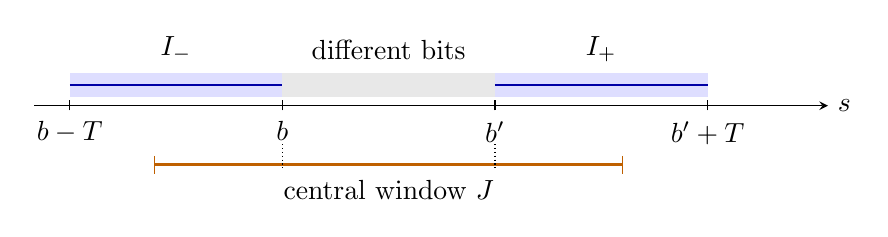
\begin{tikzpicture}[x=0.9cm,y=0.75cm,>=stealth]
 \draw[->] (-0.5,0)--(10.7,0) node[right] {$s$};
 \fill[blue!13] (0,0.15) rectangle (3,0.55);
 \fill[black!9] (3,0.15) rectangle (6,0.55);
 \fill[blue!13] (6,0.15) rectangle (9,0.55);
 \draw[blue!65!black,thick] (0,0.35)--(3,0.35);
 \draw[blue!65!black,thick] (6,0.35)--(9,0.35);
 \node at (1.5,0.95) {$I_-$};
 \node at (4.5,0.95) {different bits};
 \node at (7.5,0.95) {$I_+$};
 \foreach \x/\lab in {0/{b-T},3/{b},6/{b'},9/{b'+T}} {
  \draw (\x,-0.08)--(\x,0.1);
  \node[below] at (\x,-0.1) {$\lab$};
 }
 \draw[orange!75!black,very thick] (1.2,-1.0)--(7.8,-1.0);
 \draw[orange!75!black] (1.2,-0.85)--(1.2,-1.15);
 \draw[orange!75!black] (7.8,-0.85)--(7.8,-1.15);
 \node[below] at (4.5,-1.1) {central window $J$};
 \draw[densely dotted] (3,-0.65)--(3,-1.05);
 \draw[densely dotted] (6,-0.65)--(6,-1.05);
\end{tikzpicture}

 \caption{The intervals $I_-=[b-T,b]$ and $I_+=[b',b'+T]$, with
 $b\le b'$ and $T\ge0$, flank the bit-difference interval.
 The central window $J$ in \Cref{bud:intervals} creates excess only
 if its total overlap with the two flanks exceeds $T$; then both
 thresholds lie strictly inside $J$.}
 \label{fig:budget-intervals}
\end{figure}

\begin{proposition}[Upper score budget]\label{bud:upper}
For each $i\in\{Q,P,P\theta\}$,
\begin{equation}\label{bud:upper-equation}
 D_i\le o(S)+10\delta^2\lambda C_i.
\end{equation}
\end{proposition}

\begin{proof}
First fix a base and two distinct opposite endpoints, and write
$d,d'$ for their incident jumps.  Distinct real endpoints have
distinct $z$ coordinates, so $d\ne d'$.  At a place $v$ let
\[
 b=\min(n_e(v),n_{e'}(v)),\quad b'=\max(n_e(v),n_{e'}(v)),\quad
 u=-\log|d-d'|_v,\quad \alpha=u-b.
\]
The two opposite-endpoint coordinate differences are $d-d'$ and
$1/d-1/d'$ up to signs.  Therefore
\begin{equation}\label{bud:place-identity}
 -\log|(d-d')(1/d-1/d')|_v=2\alpha-(b'-b).
\end{equation}
All thresholds lie within the chosen level interval, so the
integrated bit-difference charge at this place is exactly $b'-b$.

Let $c_v=\log2$ at archimedean entries and $c_v=0$ otherwise.
The triangle inequality gives $\alpha\ge-c_v$, hence
$T_v:=\alpha+c_v\ge0$.  Equality of a grid label at infinity bounds
the corresponding difference by $\sqrt2$ times the grid scale;
at a finite place a matching label bounds it by the scale itself.
If both bits are $1$, a positive charge requires $s<b$ and a
$B_1$ match, which gives
\[
 s\ge b'-\alpha-c_v\ge b-T_v.
\]
If both bits are $0$, the analogous $A$ match gives
$s\ge b'$ and $s\le b+\alpha+c_v\le b'+T_v$.
Thus all positive charges lie in
\begin{equation}\label{bud:positive-intervals}
 I_-=[b-T_v,b],\qquad I_+=[b',b'+T_v].
\end{equation}
Enlarging to these full intervals is legitimate even if part of
them lies outside the chosen level interval.

Suppose a rare positive is counted with minority bit $1$ at a
threshold $s_0$.  Then $s_0<b$ and
$\Prob_E(n_e(v)>s_0)<\epsilon$.  By monotonicity every common level
and every level with minority bit $0$ lies below $s_0$; none can
produce a positive charge in $I_+$.  All minority-$1$ positive
charges lie in $I_-$ by definition.  The case of a rare positive
with minority bit $0$ is symmetric.  Thus, if any rare positive is
counted, all positive charges are on one side, their coefficients
are at most $2$, and their total is at most $2T_v$.

Otherwise only common positives remain.  For this fixed base put
\[
 J_v=\{s:(v,s)\in\mathcal C,\ |\rho(v,s)-1/2|\le\delta\}.
\]
This is an interval because the conditional edge law is fixed
across levels and both restrictions are intervals.  Extend the
coefficient $1-\lambda$ across both full intervals in
\eqref{bud:positive-intervals}, increasing it by $2\lambda$ on
$J_v$.  \Cref{bud:intervals} bounds the excess over $2T_v$ by
\[
 \lambda|J_v|\,
 \mathbf1_{\{n_e(v),n_{e'}(v)\in\operatorname{int}J_v\}}.
\]
This expression is also a valid excess bound in the rare-positive
case, when no excess is needed.  Combining it with the negative
charge and \eqref{bud:place-identity}, then summing over places,
cancels the logarithm by the product formula for the fixed nonzero
element $(d-d')(1/d-1/d')$.  The additive allowance is
$2\sum_v^*c_v=2\log2$.  Places of zero level width can be included
in this sum: their positive and negative charges vanish and the
same upper bound still holds.

Now average this bound over the fixed-base independent pair law,
restricting to distinct pairs.  Dropping that restriction only in
the nonnegative excess term, \eqref{bud:interior-mass} bounds its
expectation by $4\delta^2\lambda|J_v|$.  Boundary atoms are not
counted; distinct jumps with equal thresholds cause no exception
to this argument.  On $J_v$,
$2\rho(1-\rho)\ge2(1/4-\delta^2)$.  Averaging over bases and places
therefore bounds the distinct-pair contribution by
\[
 O(1)+\frac{4\delta^2\lambda}{2(1/4-\delta^2)}C_i
 \le O(1)+10\delta^2\lambda C_i.
\]

It remains to bound equal endpoints, to which the product formula
was not applied.  Their positive score is at most
$2(W_c+H_x^*)$ for a base vertex $x$, and their negative score is
zero.  The ordinary collision probabilities are $1/d(q)$ and
$1/d(p)$.  For templated stars \Cref{bud:pair-laws} gives the bound
$M/d(p)$ pointwise in $p$.  Consequently their total contributions
are at most, respectively,
\[
 \frac{2}{d_{Q,\min}}(W_c+\E_\kappa H_q^*),\quad
 \frac{2}{d_{P,\min}}(W_c+\E_\mu H_p^*),\quad
 \frac{2M}{d_{P,\min}}(W_c+\E_\mu H_p^*).
\]
Each is $o(S)$ by \Cref{bud:parameters,bud:rare-moments},
\eqref{bud:template-count}, and
$d_{P,\min}=t^{1+o(a)}$.  In particular multiplication by an
unbounded $H_p^*$ requires only its first moment, since the
collision estimate holds for every $p$.  Finally $O(1)=o(S)$.
\end{proof}

The upper budget is insensitive to whether the star lies at a
point or a center.  The next lower bound keeps track of that
orientation.  Its two main terms will cancel when one point-star
score is added to one center-star score.

\begin{proposition}[Rare-level lower budget]\label{bud:rare-lower}
For each of the three pair experiments, let $x$ be its star vertex
and $y$ an opposite endpoint.  Its score integrated outside
$\mathcal C$ is at least
\begin{equation}\label{bud:rare-lower-equation}
 2\E H_x^*-2\E H_y^*-o(S),
\end{equation}
where both expectations use the original edge marginals on the
appropriate sides.  In particular this is
$2\E_\kappa H_q^*-2\E_\mu H_p^*-o(S)$ for $Q$, and its opposite
main term for either $P$ or $P\theta$.
\end{proposition}

\begin{proof}
At a good rare level denote the inconsistency indicator in slot
$j$ by $M_j$.  If $I_x=1$, both other endpoints are normal, and
both edges are consistent, their dominant-coordinate labels
match each other but differ from the base's.  Both bits must
therefore be the minority bit and the required nonshared
coordinate matches.  The positive score is consequently at least
\[
 2I_x-2I_x I_{y_1}-2I_x I_{y_2}-2M_1-2M_2.
\]
If both opposite endpoints are normal and both edges consistent,
their bits agree regardless of whether the base is exceptional.
Hence the negative charge is at most
$I_{y_1}+I_{y_2}+M_1+M_2$.
Average these two pointwise bounds.  Each slot has the original
edge marginal by \Cref{bud:pair-laws}, even with templates.
The integrals of the joint terms $I_xI_{y_j}$ are $o(S)$ by
\eqref{bud:joint-exceptions}; the inconsistency integrals are
$O(1)$.  This gives \eqref{bud:rare-lower-equation} on
$\mathcal G$.  On $\mathcal B$ there are no positives and the
negative score is at least $-1$, whose total cost is
$W_b=o(S)$.
\end{proof}

\section{Common levels and positive rare mass}\label{sec:common}

We use the histories, templates and three star scores constructed in
\Cref{sec:budgets}. The first objective is to show that common levels contribute
only \(o(S)\) bit variation at a center. The second is to show that the point
exceptions on good rare levels retain a positive fraction of \(S\). Both
conclusions come from comparing the upper and lower star budgets, but the
comparison first requires a precise description of the states permitted by a
template.

Throughout this section, \(S\to\infty\), the parameters satisfy
\Cref{bud:parameters}, and \(H\) is the fixed history map from
\Cref{bud:prediction-error}. At a level, \(\nu_h\) denotes the distribution of
the true state \((A,B_1)\) of a point sampled from \(\mu\) conditional on
\(H=h\). Dependence on the level is suppressed. For a state \(y=(a,b)\), its
strict cross is
\[
 R_y=\set{(u,v):(u=a,\ v\ne b)\ \text{or}\ (u\ne a,\ v=b)}.
\]
A row means a set with fixed first coordinate; a column has fixed second
coordinate. These conventions do not refer to a geometric direction in the
plane.

\subsection{From sampled histories to the actual point}

For a center \(q\), define the mixture of predictions
\[
 \widetilde\nu_q=\E_{p\mid q}\nu_{H(p)}.
\]
For its template \(\theta=(h_1,\ldots,h_k)\), define the finite set of candidate
center states
\begin{equation}\label{com:candidates}
 \mathcal Y_\theta
 =\set{y\text{ a center state}:\nu_{h_j}(R_y)\ge1-k^{-2}
                      \text{ for every }1\le j\le k}.
\end{equation}
The actual state \(y_q\) is usually a candidate: the union bound and Markov's
inequality give, after integration on \(\mathcal C\),
\begin{equation}\label{com:actual-candidate}
 \int_{\mathcal C}\Prob(y_q\notin\mathcal Y_\theta)
 \le k^3\int_{\mathcal C}
       \E_E[1-\nu_{H(p)}(R_{y_q})]=o(S).
\end{equation}
We also need every candidate to have large mass under \(\widetilde\nu_q\).
The following elementary sampling bound supplies this uniformity.
For its first assertion, we specialize the \(\varepsilon\)-net
double-sampling argument to strict crosses
\cite[Lemmas~3.4--3.5]{HausslerWelzl1987}.
The strict-cross trace bound, the weighted-law formulation, and the subsequent
posterior-support transfer are established here.

\Needspace{5\baselineskip}
\begin{lemma}[Sampling strict crosses]\label{com:ghost}
Let \(\nu\) be a probability measure on a finite product set and let
\(X_1,\ldots,X_k\) be independent samples from \(\nu\). For
\(0<\alpha<1\) and \(k\alpha\ge8\),
\[
 \Prob\bigl(\exists y:\nu(R_y)<1-\alpha,
                    \ X_1,\ldots,X_k\in R_y\bigr)
 \le 2(2k+1)^2\,2^{-k\alpha/2}.
\]
Consequently, when \(k\) is sufficiently large, the templates in
\eqref{com:candidates} satisfy
\begin{equation}\label{com:mixture}
 \Prob\bigl(\exists y\in\mathcal Y_\theta:
              \widetilde\nu_q(R_y)<1-k^{-1/4}\mid q\bigr)
 \le 4(2k+1)^2\,2^{-k^{3/4}/2}
\end{equation}
at each level, uniformly in \(q\).
\end{lemma}

\begin{proof}
Adjoin independent samples \(X_{k+1},\ldots,X_{2k}\). If the first \(k\)
samples admit a cross as in the event, select one by a fixed ordering. For this
selected cross, the number of misses among the new samples has mean
\(k\beta\), where \(\beta=\nu(R_y^c)>\alpha\), and variance at most
\(k\beta\). Thus the probability of fewer than \(k\alpha/2\) misses is at
most \(4/(k\beta)\le1/2\). It suffices to bound twice the probability that
some cross contains the first half and misses at least \(k\alpha/2\) of the
second half.

Condition on the pooled \(2k\) samples and split their indices uniformly into
two halves. A cross induces at most \((2k+1)^2\) different subsets of these
indices: its first coordinate can agree with one of at most \(2k\) observed
coordinates, or none, and the same holds for its second coordinate. If a
pattern has \(m\) misses, the probability that they all fall in the second
half is zero for \(m>k\), and otherwise is
\[
 \frac{k(k-1)\cdots(k-m+1)}{(2k)(2k-1)\cdots(2k-m+1)}
 \le 2^{-m}.
\]
The union bound proves the first assertion. Repeated sampled states cause no
problem, since the argument concerns the indexed samples.

For the second assertion, after sampling the histories independently given
\(q\), independently sample a state from each corresponding \(\nu_{h_j}\).
Before the histories are revealed these states are independent with law
\(\widetilde\nu_q\). If a candidate violating the required conclusion exists,
select one as a function of the template. Conditional on that template, all
the synthetic states lie in its cross with probability at least
\(1-k\cdot k^{-2}=1-1/k\). Apply the first assertion with
\(\alpha=k^{-1/4}\) and divide by \(1-1/k\).
\end{proof}

Since \(W_c\le k^{1/16}S\), the integral of the failure probability in
\eqref{com:mixture} is \(o(S)\). A candidate therefore constrains the mixture
of predicted states. To constrain the actual point, we will use only rows,
columns and sets of at most two states. This restriction is essential to the
next argument.

\begin{lemma}[Transfer for restricted supports]\label{com:transfer}
Fix a level and the joint edge--template law
\[
 \Prob(p,q,\theta)=\Prob_E(p,q)\Prob(\theta\mid q).
\]
Let \(0<\eta<1/2\). As a function of \((q,\theta)\), select a support
\(U(q,\theta)\) that is a row, a column, or a set of at most two states.
On an event \(G\) determined by \((q,\theta)\), suppose
\[
 \widetilde\nu_q(U(q,\theta))\ge1-3\eta^2.
\]
Then the actual point state \(X(p)\) satisfies
\[
 \Prob\bigl(G,\ X(p)\notin U(q,\theta)\bigr)\le8\eta.
\]
The support type and its coordinates may depend on both \(q\) and \(\theta\).
\end{lemma}

\begin{proof}
Conditional on \((q,\theta)\), the history of the actual point has its
ordinary conditional law given \(q\), because the template is independent of
the point given \(q\). Hence on \(G\),
\[
 \E[\nu_{H(p)}(U(q,\theta)^c)\mid q,\theta]\le3\eta^2.
\]
The event that this support has \(\nu_{H(p)}\)-mass less than \(1-\eta\)
therefore has probability at most \(3\eta\).

For each history \(h\), define three exceptional sets using only \(\nu_h\).
If a row has mass at least \(1-\eta\), it is unique, and the first exceptional
set is its complement. If no such row exists, the first exceptional set is
empty. Define the second set in the same way for columns. Their masses are
at most \(\eta\) each.

If a set of at most two states has mass at least \(1-\eta\), put
\[
 M_h=\set{x:\nu_h(x)>\eta}
\]
and take \(M_h^c\) as the third exceptional set. Every set \(U\) of at most
two states and mass at least \(1-\eta\) contains \(M_h\): omitting an atom
of mass greater than \(\eta\) would violate that mass bound. Choosing one
such \(U\) also gives
\[
 \nu_h(M_h^c)\le\nu_h(U^c)+\nu_h(U\setminus M_h)
                 \le\eta+2\eta=3\eta.
\]
If no such \(U\) exists, the third exceptional set is empty. The union of
the three exceptional sets thus has mass at most \(5\eta\).

The actual point has marginal law \(\mu\), under which its state conditional
on \(H=h\) has distribution exactly \(\nu_h\). Consequently the probability
of this union of exceptional sets is at most \(5\eta\) under the entire
edge--template law. Outside it and the earlier nonconcentration event, the
actual state belongs to whichever permitted support was selected. Adding
the two error bounds proves the result.
\end{proof}

In the application, at most three candidates will be chosen by a fixed
ordering at each level and template. Outside the failure event bounded in
\eqref{com:mixture}, the intersection of their crosses has mixture mass at
least \(1-3k^{-1/4}\). When this intersection is contained in a row or a
column, use that row or column as \(U\); when it has size at most two, use the
intersection itself. With \(\eta=k^{-1/8}\), \Cref{com:transfer} costs at most
\[
 8k^{-1/8}W_c\le8k^{-1/16}S=o(S).
\]
An empty intersection cannot have the asserted mixture mass for large \(k\).
The proof has used the actual point marginal only for exceptional events
defined by the history and level. It has made no assertion about the law of
the actual state after additionally conditioning on a selected support.

\subsection{Classification and suppression of common variation}

We now apply this transfer to the finite geometry of strict crosses. Two
distinct center states in one row, say \((a,b)\) and \((a,b')\), have common
cross
\begin{equation}\label{com:row-intersection}
 R_{(a,b)}\cap R_{(a,b')}
       =\set{(a,v):v\notin\set{b,b'}}.
\end{equation}
A third center state outside that row cuts this intersection down to at most
one point. The corresponding assertions hold for columns. If two states
\((a,b)\) and \((a',b')\) differ in both coordinates, their common cross is
\begin{equation}\label{com:corners}
 R_{(a,b)}\cap R_{(a',b')}
       =\set{(a,b'),(a',b)}.
\end{equation}
Three states whose first coordinates are all distinct and whose second
coordinates are all distinct have empty common cross. Indeed each of the
two points in \eqref{com:corners} fails to share a coordinate with the third
state. These observations give an exhaustive classification: a candidate
set is empty, is a singleton, contains two distinct states sharing a
coordinate, or consists of states with pairwise distinct coordinates.
In the shared-coordinate case, either all candidates lie in that row or
column, or a third lies outside it. In the pairwise-distinct case there
are either two candidates or at least three.

\Cref{com:fig-crosses} shows the two-corner case: either endpoint state
together with the bit determines the state at the other endpoint.
\begin{figure}[tb]
\centering
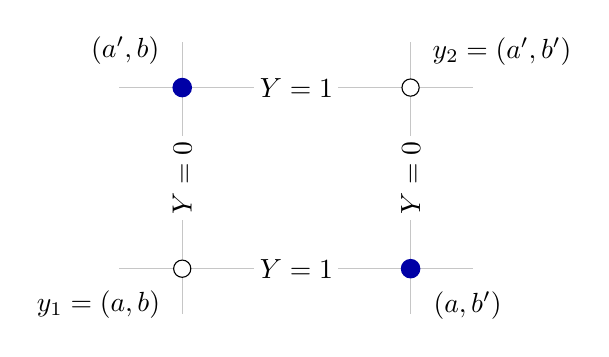
\begin{tikzpicture}[x=1.45cm,y=1.15cm]
  \draw[gray!45] (-.55,0)--(2.55,0) (-.55,2)--(2.55,2);
  \draw[gray!45] (0,-.5)--(0,2.5) (2,-.5)--(2,2.5);
  \node[draw,circle,fill=white,inner sep=2.2pt] (y1) at (0,0) {};
  \node[draw,circle,fill=white,inner sep=2.2pt] (y2) at (2,2) {};
  \node[circle,fill=blue!65!black,inner sep=2.5pt] (x1) at (2,0) {};
  \node[circle,fill=blue!65!black,inner sep=2.5pt] (x2) at (0,2) {};
  \node[below left=3pt of y1] {\(y_1=(a,b)\)};
  \node[above right=3pt of y2] {\(y_2=(a',b')\)};
  \node[below right=3pt of x1] {\((a,b')\)};
  \node[above left=3pt of x2] {\((a',b)\)};
  \node[rotate=90,fill=white,inner sep=2pt] at (0,1) {\(Y=0\)};
  \node[rotate=90,fill=white,inner sep=2pt] at (2,1) {\(Y=0\)};
  \node[fill=white,inner sep=2pt] at (1,0) {\(Y=1\)};
  \node[fill=white,inner sep=2pt] at (1,2) {\(Y=1\)};
\end{tikzpicture}
\caption{Two candidate center states differing in both coordinates admit
exactly two point states in their common strict cross. The filled points are
those opposite corners. Within this four-state configuration, the bit of a
consistent edge and the state at either endpoint determine the state at
the other endpoint. Rows have fixed first label and columns have fixed
second label. The diagram displays coordinate
equalities of states, not geometric positions of the original plane points.}
\label{com:fig-crosses}
\end{figure}


Declare a single edge with its template bad at a common level if its state
test is inconsistent, if \(y_q\notin\mathcal Y_\theta\), if
the event inside the probability in \eqref{com:mixture} occurs, or if the
restricted-support transfer fails for
the witnesses specified by this classification. The witnesses are two
states sharing a coordinate, with a third outside that row or column when
one exists; two states differing in both coordinates; or three states with
pairwise distinct coordinates. Empty candidate sets and empty witness
intersections have no good edges. All choices are deterministic functions
of the level and template. The preceding estimates and the integrated
inconsistency bound give
\begin{equation}\label{com:bad-mass}
 \int_{\mathcal C}\Prob(p,q,\theta\text{ is bad})=o(S).
\end{equation}

The comparisons below must use the full conditional bit probability
\(\rho\) in the definition of the scores. We never remove bad edges and
renormalize that law. In particular the discontinuity of \(c(\rho)\) at
\(1/2\pm\delta\) introduces no error.

Here is the numerical estimate used in the two-corner case. For every
\(0\le\rho\le1\), with \(\delta=0.01\), \(\lambda=\delta^2/2\), and
\(c\) as in \Cref{sec:budgets},
\begin{align}
 c(\rho)\bigl(\rho^2+(1-\rho)^2\bigr)-2\rho(1-\rho)
 &= (2\rho-1)^2+
       (c(\rho)-1)\bigl(\rho^2+(1-\rho)^2\bigr)\notag\\
 &\ge\lambda/2.\label{com:score-polynomial}
\end{align}
For \(\abs{\rho-1/2}\le\delta\), discard the first square and use
\(\rho^2+(1-\rho)^2\ge1/2\). Outside that interval the expression is at
least \(4\delta^2-\lambda>\lambda/2\).

\Needspace{5\baselineskip}
\begin{proposition}[Common variation]\label{com:variation}
For the center-star and point--template-star experiments of
\Cref{bud:pair-laws},
\begin{equation}\label{com:variation-eq}
 C_Q+C_{P\theta}=o(S).
\end{equation}
Moreover their rare exception means satisfy
\begin{equation}\label{com:center-rare}
 \E_\kappa H_q^*\le\E_\mu H_p^*+o(S).
\end{equation}
\end{proposition}

\begin{proof}
Fix a common level. For each template of positive probability, let
\(\pi_\theta=\Prob(\theta)\) and
\(b_\theta=\Prob(\text{bad edge}\mid\theta)\), with both probabilities taken
under the joint law in \Cref{com:transfer}. In the center-star experiment,
condition on \(\theta\) and then sample \(q\) by its actual conditional law.
The two points are still independent with their ordinary law given \(q\).
In the point--template-star experiment, sample \(p\) conditional on
\(\theta\), then two independent centers given \((p,\theta)\). Each slot
in either experiment has the same conditional single-edge law
\(\Prob(p,q\mid\theta)\). Therefore a pair with at least one bad slot has
probability at most \(2b_\theta\) in either experiment.

Write \(V_Q(\theta)\) and \(V_{P\theta}(\theta)\) for the corresponding
averages of \(2\rho(1-\rho)\) over bases in this slice, and write
\(d_Q(\theta),d_{P\theta}(\theta)\) for its two common-level expected
scores. Each \(V\) is at most \(1/2\), and either score is at least the
negative of its variation. We prove
\begin{equation}\label{com:slice-score}
 d_Q(\theta)+d_{P\theta}(\theta)
 \ge\frac\lambda4\bigl(V_Q(\theta)+V_{P\theta}(\theta)\bigr)
       -C b_\theta
\end{equation}
with an absolute constant \(C\). All coefficients in a common score are
bounded by \(1+\lambda\), so charging a pair with a bad slot always costs
at most an absolute multiple of its probability.

\emph{An empty candidate set.}
Every edge is bad, so \(b_\theta=1\), and the boundedness of the scores proves
\eqref{com:slice-score} on increasing \(C\).

\emph{One candidate state.}
At a fixed point--template base, two good edges have the same center state.
Consistency forces their bits to agree, and the nonshared coordinate of
their center states matches. Thus this star score is at least
\(1-\lambda-O(b_\theta)\) after averaging over its bases. The center-star
score is at least \(-1/2\). Their sum is at least
\(1/2-\lambda-O(b_\theta)\), which implies \eqref{com:slice-score} because
the two variations sum to at most one.

\emph{Two candidates sharing a coordinate, and all candidates in that row
or column.}
The transfer using \eqref{com:row-intersection} places every good point in
the same row or column. If it is a row, every good edge has matching
\(A\)-coordinates and hence bit \(1\), by consistency; in the column case
every good edge has bit \(0\). A bit difference in either pair experiment
therefore requires a bad slot. This gives
\(V_Q(\theta)+V_{P\theta}(\theta)\le4b_\theta\). The lower score bound
\(d_i\ge-V_i\) now proves \eqref{com:slice-score}.

\emph{Two candidates sharing a coordinate, and a third outside that row
or column.}
The three witness crosses intersect in at most one state. If the
intersection is empty, all edges are bad. Otherwise all good point states
equal that one state. At a center base, two good edges consequently have
equal bits and the required nonshared-coordinate match. Its score is at
least \(1-\lambda-O(b_\theta)\), and the other score is at least \(-1/2\).
The same estimate as in the singleton case applies.

\emph{No coordinate shared by distinct candidates.}
If there are at least three candidates, their common cross is empty and
all edges are bad. Otherwise there are exactly two candidates. The good
point states lie in their two opposite corners from \eqref{com:corners}.
At either type of base, a good edge's bit determines the state at the other
endpoint. Thus two good edges with equal bits have the required collision.
For the full conditional probability \(\rho\) at that base, their expected
score is at least the left side of \eqref{com:score-polynomial}, less an
absolute multiple of the probability of a bad slot. After averaging bases,
each score is at least \(\lambda/2-O(b_\theta)\), which proves
\eqref{com:slice-score}.

This completes the classification. Multiply \eqref{com:slice-score} by its
actual slice weight \(\pi_\theta\), sum, and integrate over common levels.
The error is
\(C\int_{\mathcal C}\sum_\theta\pi_\theta b_\theta=o(S)\) by
\eqref{com:bad-mass}. This argument allows individual \(b_\theta\) to be
large; no inverse slice weight or number of templates enters. The common
contributions to \(D_Q+D_{P\theta}\) are therefore at least
\[
 \frac\lambda4(C_Q+C_{P\theta})-o(S).
\]
The lower bounds in \Cref{bud:rare-lower} outside common levels cancel their
main terms, because the two star vertices are on opposite sides. Hence
\[
 \frac\lambda4(C_Q+C_{P\theta})-o(S)
 \le D_Q+D_{P\theta}
 \le 10\delta^2\lambda(C_Q+C_{P\theta})+o(S),
\]
where the last inequality is \Cref{bud:upper}. Since
\(10\delta^2<1/4\), this proves \eqref{com:variation-eq}.

Finally the common contribution to \(D_Q\) is at least \(-C_Q\).
\Cref{bud:rare-lower} and \Cref{bud:upper} therefore give
\[
 2\E_\kappa H_q^*-2\E_\mu H_p^*-C_Q-o(S)
 \le D_Q\le10\delta^2\lambda C_Q+o(S).
\]
Use \(C_Q=o(S)\) to obtain \eqref{com:center-rare}.
\end{proof}

\subsection{A second score forces positive rare mass}

We have suppressed common variation at centers. To show that point exceptions
remain on rare levels, suppose temporarily that their mean is \(o(S)\).
\Cref{com:variation} then gives the same bound for center exceptions. We will
show that common variation is also small at ordinary point stars. Once both
ordinary star variations are small, expansion forces the edge bit itself to
be almost constant at nearly every level, contradicting \(S=\int f\).

For a probability measure \(\nu\) on states, let \(\nu_A,\nu_{B_1}\) denote
its coordinate marginals, with squared norms equal to the sums of squares of
their atom masses. Define
\begin{equation}\label{com:T}
 T=\int_{\mathcal C}\E_\mu\left[
       \norm{(\nu_{H(p)})_A}_2^2+
       \norm{(\nu_{H(p)})_{B_1}}_2^2-1\right].
\end{equation}
These norms count coordinate matches between two independent predicted
points with the same history. Unlike the preceding star scores, \(T\) uses
no center.

\begin{lemma}[The two-prediction score]\label{com:prediction-score}
If \(\E_\mu H_p^*=o(S)\), then \(T\le o(S)\).
\end{lemma}

\begin{proof}
Choose a history with its marginal probability, then two independent points
\(p',p''\) from \(\mu\) conditional on that history. This is one fixed
coupling throughout all levels, and each point marginal is \(\mu\). At a
level, the expected value of
\[
 F(p',p'')=
   \1_{\{A(p')=A(p'')\}}+
   \1_{\{B_1(p')=B_1(p'')\}}-1
\]
is the integrand in \eqref{com:T}.

For a distinct pair put \(Z=z_{p'}-z_{p''}\) and
\(W=w_{p'}-w_{p''}\), both nonzero. At a place with level interval
\([l,u]\), the endpoint conditions from \eqref{ht:range} say
\(l\le-\log|Z|_v\) and \(u\ge\log|W|_v\). The \(A\)-match can hold only
for \(s\le-\log|Z|_v+O_v(1)\), and the \(B_1\)-match only for
\(s\ge\log|W|_v-O_v(1)\). Here the constants vanish at nonarchimedean
places and are absolute at infinity. Therefore
\[
 \int_l^u F(p',p'')\dd s
 \le-\log|Z|_v-\log|W|_v+O_v(1).
\]
The product formula, and total archimedean weight one, show that the
integral over all levels is at most an absolute constant.

At a good rare level where neither point is exceptional, their dominant
coordinate labels match, so \(F\ge0\). In general at such a level
\[
 F\ge-\1_{\{p'\text{ exceptional}\}}-
         \1_{\{p''\text{ exceptional}\}}.
\]
The contribution on damaged levels is at least \(-W_b\). Removing all
noncommon levels from the full integral consequently gives, for each
distinct pair,
\[
 \int_{\mathcal C}F(p',p'')
       \le O(1)+H_{p'}^*+H_{p''}^*+W_b.
\]

On the diagonal the common-level integral is exactly \(W_c\). Its
probability under the selected coupling is
\[
 \sum_{p\in P}\frac{\mu(p)^2}{\mu(H^{-1}(H(p)))}
 \le |H(P)|\max_p\mu(p)=t^{-1+o(1)}.
\]
Here \(|H(P)|\le L^{2K}=t^{o(1)}\) and the marginal degree bounds were
proved in \Cref{sec:incidence}. Since
\(W_c\le k^{1/16}S\) and \(k=t^{o(1)}\), its contribution is \(o(S)\).
Average the bound for distinct pairs, using the two marginals \(\mu\),
\(W_b=o(S)\), and \(S\to\infty\). This proves
\(T\le2\E_\mu H_p^*+o(S)=o(S)\).
\end{proof}

\begin{proposition}[Positive rare mass]\label{com:rare-positive}
The good rare point exceptions satisfy
\begin{equation}\label{com:rare-positive-eq}
 \liminf_{t\to\infty}\frac{\E_\mu H_p^*}{S}>0.
\end{equation}
\end{proposition}

\begin{proof}
If the conclusion fails, restrict to a subsequence on which
\(\E_\mu H_p^*=o(S)\). By \eqref{com:center-rare}, also
\(\E_\kappa H_q^*=o(S)\), and \Cref{com:prediction-score} gives
\(T\le o(S)\).

At a common level declare an ordinary edge bad if its test is inconsistent
or if
\(\nu_{H(p)}(R_{y_q})<1-k^{-2}\). Its integrated probability is \(o(S)\),
because Markov's inequality bounds the second contribution by
\(k^2\int_{\mathcal C}\E_E[1-\nu_{H(p)}(R_{y_q})]=o(S)\).
Fix a point \(p\) and this level. Write \(b_p\) for its conditional bad-edge
probability, \(\nu=\nu_{H(p)}\), \(\zeta=k^{-2}\), and
\[
 \tau(\nu)=\norm{\nu_A}_2^2+\norm{\nu_{B_1}}_2^2-1.
\]
Let \(\mathcal Y_p\) be the states of its good neighbors. Every such state
has \(\nu(R_y)\ge1-\zeta\), and the actual point state belongs to each
\(R_y\), by consistency. Let \(d_P(p)\) be the common-level score at this
ordinary point star, using its full bit probability \(\rho_p\). We claim
\begin{equation}\label{com:second-slice-score}
 d_P(p)+\tau(\nu)
 \ge\frac\lambda4\,2\rho_p(1-\rho_p)-C(b_p+\zeta).
\end{equation}
As before, a pair with a bad slot costs only \(O(b_p)\); its probability is
at most \(2b_p\). The strict-cross classification proves the claim as
follows.

If \(\mathcal Y_p\) is empty, \(b_p=1\), while \(d_P(p)\ge-1/2\) and
\(\tau(\nu)\ge-1\), so the claim holds for an absolute \(C\).

If \(\mathcal Y_p=\set{(a,b)}\), put
\(r=\nu_A(a)\), \(s=\nu_{B_1}(b)\). Since
\(r+s\ge\nu(R_{(a,b)})\ge1-\zeta\),
\[
 \tau(\nu)\ge r^2+s^2-1
        \ge\tfrac12(1-\zeta)^2-1\ge-\tfrac12-\zeta.
\]
Two good neighbors have the same state and bit, so
\(d_P(p)\ge1-\lambda-O(b_p)\). Their sum has the positive lower bound
needed for \eqref{com:second-slice-score}.

If two states share a row, their common cross is in that row, of
\(\nu\)-mass at least \(1-2\zeta\). Thus
\(\tau(\nu)\ge(1-2\zeta)^2-1\ge-4\zeta\).
If every state is in that row, the actual point lies there too, since it
belongs to the crosses of both distinct states. All good edges consequently
have bit \(1\). Their full-law variation is at most \(2b_p\), and
\(d_P(p)\ge-2b_p\), proving the claim in this case. Columns give bit \(0\)
and the same estimates. If there is a third state outside the row or column,
the three crosses have intersection of size at most one and mass at least
\(1-3\zeta\). It must be a singleton for large \(k\). Both marginals then
have an atom of at least that mass, giving
\[
 \tau(\nu)\ge2(1-3\zeta)^2-1\ge1-12\zeta.
\]
Together with \(d_P(p)\ge-1/2\), this is more than sufficient.

Finally suppose no coordinate is shared by distinct states in
\(\mathcal Y_p\). Three such states are impossible, since the actual point
belongs to all their crosses and their intersection is empty. In the
remaining case there are two states differing in both coordinates. The two
opposite corners carry \(\nu\)-mass at least \(1-2\zeta\). Each coordinate
marginal therefore has at least that mass on a set of size two, so
\[
 \tau(\nu)\ge
  2\cdot\frac{(1-2\zeta)^2}{2}-1\ge-4\zeta.
\]
The actual point is one of those corners. Its bit determines the good
neighbor state; hence \eqref{com:score-polynomial} gives
\(d_P(p)\ge\lambda/2-O(b_p)\). This completes the proof of
\eqref{com:second-slice-score}.

Average \eqref{com:second-slice-score} over \(p\) and integrate on common
levels. The bad-edge integral is \(o(S)\), and
\(\zeta W_c\le k^{-31/16}S=o(S)\). The result is
\[
 (\text{common contribution to }D_P)+T
       \ge\frac\lambda4 C_P-o(S).
\]
The noncommon contribution to \(D_P\) is at least \(-o(S)\) by
\Cref{bud:rare-lower}, under the present assumptions on both exception
means. Therefore
\[
 \frac\lambda4 C_P-o(S)
 \le D_P+T\le10\delta^2\lambda C_P+o(S),
\]
and again \(10\delta^2<1/4\) yields \(C_P=o(S)\).

To finish, let \(V_P,V_Q\) be the ordinary star variations at any fixed
level. Assign to each vertex its conditional majority bit, breaking ties
in a fixed way. The probability that the bit on an incident edge differs
from this label is at most the corresponding average variation, because
\(\min(\rho,1-\rho)\le2\rho(1-\rho)\). Thus the two endpoint labels disagree
on an edge with probability at most \(V_P+V_Q\). When that sum is small,
the matching-label consequence of expansion in \Cref{inc:matching} gives
one bit label with total marginal exception probability
\(O(V_P+V_Q)\). The edge bit differs from it with probability
\(O(V_P+V_Q)\) as well. When the sum is not small the same bound follows
from \(f\le1/2\), with a larger absolute constant. Consequently
\[
 f\le C(V_P+V_Q)
\]
uniformly for all sufficiently large \(t\). Integrating on common levels
gives \(\int_{\mathcal C}f\le C(C_P+C_Q)=o(S)\).

On good rare levels, the minority-bit probability is bounded by the two
marginal exception probabilities and the inconsistency probability, as in
\Cref{bud:rare-moments}. Its integral is \(o(S)\) under the present
assumptions. Damaged levels contribute at most \(W_b/2=o(S)\). Thus
\(S=\int f=o(S)\), a contradiction. This proves
\eqref{com:rare-positive-eq}.
\end{proof}

The positive rare mass is a first-moment statement. To extract many
pairs at a single height scale, \Cref{sec:extraction} next controls its
large-height tail and removes errors in height-weighted measure before
selecting a band. Throughout that selection, the center-star variation
bound $C_Q=o(S)$ remains available under the original wedge law.

\section{Extracting multiplicatively organized pairs}\label{sec:extraction}

We now use \Cref{com:variation,com:rare-positive}: the ordinary center-star
variation satisfies \(C_Q=o(S)\), whereas the point exception mass satisfies
\(\liminf \E_\mu H_p^*/S>0\).  Here \(S\to\infty\), and the parameters,
levels, and exception indicators are those of \Cref{sec:budgets}.
Our objective is a graph on two copies of \(P\) whose edges carry ratios of
unit jumps.  These ratios will have large height, while their alternating
products around every complete rectangle have negligible height.

Throughout this section an \emph{ordinary wedge} is sampled by taking
\(q\) with law \(\kappa\) and then taking \(p,r\) independently and uniformly
among its neighbors in \(E\).  Its two point marginals are \(\mu\).
We retain the notation \(W_c\) for the width of common levels, \(W_b\) for
the width of damaged rare levels, and \(m_{pq}\) for the integrated
inconsistency indicator of the edge \(pq\).  In particular,
\begin{equation}\label{ext:inputs}
 \E_\mu H_p^*+\E_\kappa H_q^*=O(S),\qquad
 \E_E m_{pq}=O(1),\qquad
 W_c\le S/\epsilon,\qquad W_b=o(S),
 \quad \epsilon=k^{-1/16}.
\end{equation}
All integrals over levels include the prescribed place weights.

\subsection{A pointwise estimate and its tail consequence}

The first-moment bound in \eqref{ext:inputs} alone does not prevent all
exception mass from being carried by extremely rare points.  We obtain the
needed tail control by applying the product formula separately to each
distinct pair of neighbors of a point.

\begin{lemma}[Pointwise rare-level estimate]\label{ext:pointwise}
For every \(p\in P\) and every pair of distinct neighbors \(q,q'\in Q\),
\begin{equation}\label{ext:pointwise-bound}
 2H_p^*\le
 3\bigl(H_q^*+H_{q'}^*+m_{pq}+m_{pq'}\bigr)
       +W_c+W_b+2\log 2.
\end{equation}
\end{lemma}

\begin{proof}
At a good rare level, let \(X,U,V\) be the exception indicators of
\(p,q,q'\), and let \(I,I'\) be the inconsistency indicators of the two
edges.  Write \(P_+\) for the rare positive charge in the point-star score:
it equals two when \(p\) is exceptional, both bits are minority bits, and
the two neighbors have matching nonshared coordinates; otherwise it is
zero.  Write \(N=\abs{Y_{pq}-Y_{pq'}}\).
If \(U=V=I=I'=0\), the two bits are the same function of \(X\): they are
both majority bits for \(X=0\), and both minority bits for \(X=1\).
In the latter case the nonshared coordinate of both neighbors has the
dominant label, so \(P_+=2\).  Consequently, pointwise,
\[
 P_+\ge 2X-2(U+V+I+I'),\qquad
 N\le U+V+I+I',
\]
and hence
\begin{equation}\label{ext:local-rare-score}
 P_+-N\ge 2X-3(U+V+I+I').
\end{equation}
In particular, a simultaneous exception at \(p\) and at a neighbor is
charged directly to the neighbor indicator.

For completeness, the upper bound for this rare-only score is also
pointwise.  Put \(d=z_p-z_q\), \(d'=z_p-z_{q'}\).  These jumps are distinct
and nonzero.  At a place \(v\), sort their thresholds as \(b\le b'\), and set
\[
 u=-\log\abs{d-d'}_v,\qquad \alpha=u-b,\qquad
 T_v=\begin{cases}\alpha+\log 2,&v\text{ archimedean},\\
                    \alpha,&v\text{ nonarchimedean}.
       \end{cases}
\]
The triangle inequality makes \(T_v\ge0\).  Matching coordinates in a
square cell of side length \(r\) gives distance at most \(\sqrt2 r\), and
matching nonarchimedean labels gives distance at most \(r\).
Thus positive charges with both bits one lie within \([b-T_v,b]\), and
positive charges with both bits zero lie within \([b',b'+T_v]\).

Only one of these two intervals can contain a rare positive charge.
Indeed every level where zero is the minority bit precedes every level
where one is the minority bit.  A zero-bit rare positive would require a
threshold at least \(b'\), while a one-bit rare positive would require a
later threshold strictly less than \(b\), which is impossible.
The total rare positive charge at this place is therefore at most
\(2T_v\).  The all-level negative charge is \(b'-b\), because the level
interval contains both thresholds.  Moreover,
\[
 -\log\abs{(d-d')(1/d-1/d')}_v=2\alpha-(b'-b).
\]
Summing over places, the product formula cancels this last expression.
The archimedean weights sum to one, so the rare positives minus the
all-level negative charge total at most \(2\log2\).

Integrating \eqref{ext:local-rare-score} gives a lower bound for that same
score.  Outside the good rare levels there are no positive terms, and
the negative charge is at most \(W_c+W_b\).  Comparing the lower and upper
bounds proves \eqref{ext:pointwise-bound}.
\end{proof}

\begin{lemma}[Tail control]\label{ext:tail}
Let \(R_0=\epsilon^{-2}=k^{1/8}\).  Then
\begin{equation}\label{ext:tail-bound}
 \E_\mu\bigl[H_p^*\mathbf1_{\{H_p^*>R_0S\}}\bigr]=o(S).
\end{equation}
\end{lemma}

\begin{proof}
Choose an absolute \(C_0\) for which each of the two exception expectations
in \eqref{ext:inputs} is at most \(C_0S\), for all sufficiently large
indices.  Put
\[
 T=\{p:H_p^*>R_0S\},\qquad
 A_t=\E_\mu[H_p^*\mathbf1_T],\qquad
 d_{P,\min}=\min_{p\in P}d(p).
\]
On \(T\), the deterministic last three terms of
\eqref{ext:pointwise-bound} have sum at most \(H_p^*\), eventually, since
\[
 \frac{W_c+W_b+2\log2}{R_0S}
 \le\epsilon+\frac{W_b+2\log2}{R_0S}=o(1).
\]
After absorbing them, we may cap each neighbor height at \(H_p^*\):
\begin{equation}\label{ext:capped-pointwise}
 H_p^*\le3\bigl(\min(H_p^*,H_q^*)+\min(H_p^*,H_{q'}^*)
                       +m_{pq}+m_{pq'}\bigr),\qquad p\in T,
\end{equation}
for distinct \(q,q'\).  If a cap changes a term, that capped term already
equals \(H_p^*\) and suffices for this inequality; otherwise the preceding
inequality is unchanged.

Sample \(p\) with law \(\mu\) and two neighbors independently and uniformly
given \(p\).  Restrict the left side to distinct neighbors.  The exact
conditional probability of distinctness is \(1-1/d(p)\).  On the
nonnegative right side we can drop this restriction.  Thus
\begin{equation}\label{ext:tail-average}
 (1-d_{P,\min}^{-1})A_t
 \le 6\E_E[\min(H_p^*,H_q^*)\mathbf1_T]+C_m,
\end{equation}
where \(C_m\) is an absolute upper bound for \(6\E_E m_{pq}\).
This calculation uses the distinctness probability at each individual
point, so it remains valid even when its exception mass is very large.

We estimate the capped expectation by layer cake.  For \(u\ge0\) let
\[
 F_u=\{p:H_p^*>\max(u,R_0S)\},\qquad
 G_u=\{q:H_q^*>u\},
\]
and write \(h_P(u)=\mu(F_u)\), \(h_Q(u)=\kappa(G_u)\).
The marginal version of the expansion estimate from \Cref{sec:incidence},
with \(\eta=\gamma-1/2>0\), is
\[
 \Prob_E(F,G)\le\sqrt{\mu(F)\kappa(G)}
 \left[\gamma^{-(1+2\eta)}(\mu(F)\kappa(G))^\eta
                         +\gamma^{-1}\xi_t\right].
\]
Because \(h_P(u)\le C_0/R_0\) and \(h_Q(u)\le1\), the same multiplier
\[
 \vartheta_t=\gamma^{-(1+2\eta)}(C_0/R_0)^\eta
                      +\gamma^{-1}\xi_t=o(1)
\]
works at every threshold \(u\), including thresholds where the center set
has full measure.  Tonelli's theorem and Cauchy--Schwarz now give
\begin{align*}
 \E_E[\min(H_p^*,H_q^*)\mathbf1_T]
 &=\int_0^\infty\Prob_E(F_u,G_u)\dd u\\
 &\le\vartheta_t
       \left(\int_0^\infty h_P(u)\dd u\right)^{1/2}
       \left(\int_0^\infty h_Q(u)\dd u\right)^{1/2}\\
 &=\vartheta_t\sqrt{A_t\E_\kappa H_q^*}
 \le\vartheta_t\sqrt{C_0A_tS}.
\end{align*}
The first integral equals the unknown tail first moment \(A_t\), including
its contribution below the threshold \(R_0S\).
Since \(d_{P,\min}\to\infty\), \eqref{ext:tail-average} implies eventually
\[
 \tfrac12 A_t\le6\vartheta_t\sqrt{C_0A_tS}+C_m
       \le\tfrac14 A_t+36C_0\vartheta_t^2S+C_m.
\]
The last step is Young's inequality.  Consequently
\[
 \frac{A_t}{S}\le144C_0\vartheta_t^2+\frac{4C_m}{S}\longrightarrow0,
\]
as required.
\end{proof}

\subsection{Point profiles and a common height band}

We next express a wedge's jump ratio as a difference of profiles attached
to its two point endpoints.  On a good rare level \((v,s)\), let
\(X_x(v,s)=I_x(v,s)\) be the exception indicator of the vertex \(x\)
from \Cref{sec:budgets}, and let
\(\sigma(v,s)=1\) when one is the minority bit and \(-1\) when zero is
the minority bit.  Define a real-valued profile, indexed by places, by
\begin{equation}\label{ext:profile-definition}
 a_p(v)=\int_{\substack{s:\,(v,s)\text{ is}\\\text{good rare}}}
                       \sigma(v,s)X_p(v,s)\dd s.
\end{equation}
For a place profile \(b\), write \(\norm{b}_1=\sum_v^*\abs{b(v)}\).

\begin{lemma}[Wedge profiles]\label{ext:profiles}
For an ordinary wedge \((p,q,r)\), there are nonnegative random variables
\(E_1,E_2\), with \(\E E_1+\E E_2=o(S)\), such that
\begin{align}
 \norm{(n_{pq}-n_{rq})-(a_p-a_r)}_1&\le E_1,
                                      \label{ext:profile-error}\\
 \norm{n_{pq}-n_{rq}}_1&\ge H_p^*+H_r^*-E_2.
                                      \label{ext:profile-size}
\end{align}
Here \(n_{pq}(v)=-\log\abs{z_p-z_q}_v\).
\end{lemma}

\begin{proof}
Let \(\mathcal G\) denote the good rare levels, and let \(I_{pq}\) be
the levelwise inconsistency indicator.  At a level in \(\mathcal G\),
write \(b\in\{0,1\}\) for the majority bit.  Consistency gives
\[
 Y_{pq}=b+\sigma(X_p+X_q)
\]
unless both endpoints are exceptional or the edge is inconsistent.
In all cases the absolute residual in this identity is at most
\(2(X_pX_q+I_{pq})\).  Subtracting the identities for the two edges
cancels the center contribution.  At each place,
\[
 n_{pq}(v)-n_{rq}(v)=\int(Y_{pq}-Y_{rq})\dd s,
\]
since both bits are single thresholds inside the level interval.
It follows that \eqref{ext:profile-error} holds with
\[
 E_1=\int_{\mathcal C}\abs{Y_{pq}-Y_{rq}}+W_b
       +2\int_{\mathcal G}(X_pX_q+X_rX_q+I_{pq}+I_{rq}).
\]
Its mean is \(o(S)\): the first term averages to \(C_Q=o(S)\), the
joint edge exceptions have integrated expectation \(o(S)\), and the
remaining bounds are in \eqref{ext:inputs}.

There is also the exact identity
\[
 \norm{n_{pq}-n_{rq}}_1=\int\abs{Y_{pq}-Y_{rq}}.
\]
On a good rare level with exactly one exceptional point endpoint, a
normal center, and two consistent edges, the bits differ.  More
explicitly, at every good rare level,
\[
 \abs{Y_{pq}-Y_{rq}}\ge X_p+X_r
 -2(X_pX_r+X_pX_q+X_rX_q+I_{pq}+I_{rq}).
\]
If none of the terms subtracted is present, this is the preceding
observation; if any is present, the right side is nonpositive.
Integrating proves \eqref{ext:profile-size} with
\[
 E_2=2\int_{\mathcal G}
                   (X_pX_r+X_pX_q+X_rX_q+I_{pq}+I_{rq}).
\]
The integrated joint point exceptions on a wedge and joint edge
exceptions are \(o(S)\), by \Cref{bud:rare-moments}.
Thus \(\E E_2=o(S)\) as well.
\end{proof}

The next selection makes these average error bounds uniform before
choosing a dyadic band.  This order matters because the probability of
the eventual band tends to zero.

\begin{lemma}[A band of accurate wedges]\label{ext:band}
There are a constant \(c>0\), independent of \(t\) along the fixed
sequence, a sequence \(\delta_t\to0\), and scales \(J\to\infty\) such
that a set of ordinary wedges of probability at least
\begin{equation}\label{ext:band-mass}
 \frac{c}{R_0\log(2R_0)}=t^{-o(1)}
\end{equation}
satisfies, uniformly on the set,
\begin{equation}\label{ext:band-conditions}
 J\le H_p^*+H_r^*\le2J,\qquad
 E_1+E_2\le\delta_t(H_p^*+H_r^*).
\end{equation}
Every such wedge has \(p\ne r\).
\end{lemma}

\begin{proof}
Set \(W=H_p^*+H_r^*\) and \(Z=E_1+E_2\).  By
\Cref{com:rare-positive}, choose \(c_0>0\), independent of \(t\) along
the fixed sequence, such that \(\E W\ge4c_0S\) eventually.
Choose \(\delta_t\to0\) sufficiently
slowly that \(\E Z/\delta_t=o(S)\).  Before selecting any band, discard
wedges with \(Z>\delta_tW\).  Their lost weight is at most
\[
 \E[W\mathbf1_{\{Z>\delta_tW\}}]\le\frac{\E Z}{\delta_t}=o(S).
\]
Also discard \(W<c_0S\), losing at most \(c_0S\).
If \(W>2R_0S\), its larger summand exceeds \(R_0S\) and is at least
\(W/2\).  Thus \Cref{ext:tail} gives
\[
 \E[W\mathbf1_{\{W>2R_0S\}}]
 \le2\E[H_p^*\mathbf1_{\{H_p^*>R_0S\}}]
    +2\E[H_r^*\mathbf1_{\{H_r^*>R_0S\}}]=o(S).
\]
The surviving weighted mass is at least \(2c_0S\), whereas every
surviving wedge has \(W\le2R_0S\).  Its probability is therefore at
least \(c_0/R_0\).

Partition \([c_0S,2R_0S]\) into at most
\(1+\lceil\log_2(2R_0/c_0)\rceil=O(\log(2R_0))\) dyadic bands,
using half-open endpoints except at the final endpoint.  One band has
the probability in \eqref{ext:band-mass}; if \(J\) is its lower endpoint,
then \(J\ge c_0S\to\infty\), and \eqref{ext:band-conditions} holds.
The parameter hierarchy gives \(k=t^{o(1)}\), so the lower bound in
\eqref{ext:band-mass} is indeed \(t^{-o(1)}\).
Finally, if \(p=r\), the left side of \eqref{ext:profile-size} is zero,
whereas its right side is at least \((1-\delta_t)W>0\) for all
sufficiently large indices.  Such a wedge cannot survive.
\end{proof}

\subsection{Removing common unit circles and choosing witnesses}

The algebraic argument will require that a retained pair does not lie
on a common unit circle containing many points of \(P\).  This exclusion
must concern all real unit circles, including those whose centers do
not belong to \(Q\).

\begin{lemma}[Popular-circle deletion]\label{ext:circles}
Call a real unit circle \emph{popular} if it contains at least
\(t^{9/10}\) points of \(P\).  The ordinary wedge probability of
\(p,r\) lying on a common popular circle is at most
\begin{equation}\label{ext:circle-cost}
 t^{-3/5+o(1)}+t^{-9/5+o(1)}+\frac{2}{\min_{q\in Q}d(q)}.
\end{equation}
This is \(o(1/(R_0\log(2R_0)))\).  In particular, removing such wedges
from the set in \Cref{ext:band} preserves the lower probability bound
\eqref{ext:band-mass}, after decreasing its constant.
\end{lemma}

\begin{proof}
Write \(M\) for the number of popular circles.  Every pair of distinct
real points lies on at most two unit circles.  Counting pairs on popular
circles therefore gives
\[
 M\binom{\lceil t^{9/10}\rceil}{2}
 \le2\binom{\abs P}{2},\qquad M\le t^{1/5+o(1)},
\]
using \(\abs P=t^{1+o(1)}\).
The set \(P_{\rm mult}\) of points on at least two popular circles has
size at most \(2\binom M2\le t^{2/5+o(1)}\), because distinct circles
intersect in at most two points.  The degree bounds give
\[
 \max_p\mu(p)\le t^{-1+o(1)},\qquad
 \max_q\kappa(q)\le t^{-2+o(1)}.
\]
Consequently wedges hitting \(P_{\rm mult}\) at either point endpoint
have probability at most \(t^{-3/5+o(1)}\).  Centers in \(Q\) whose
own unit circle is popular number at most \(M\); wedges with such a
center have probability at most \(t^{-9/5+o(1)}\).

To bound the remaining bad wedges, fix \(p\notin P_{\rm mult}\) and
a center \(q\) whose own circle is not popular, in the original sampling
law.  The point \(p\) belongs to at most one popular circle.  If there is
one, it differs from the unit circle centered at \(q\), since the
latter is not popular.  Their intersection has at most two points.
In this original law, \(r\) is a uniform neighbor of \(q\), so the
probability that it shares a popular circle with \(p\) is at most
\(2/d(q)\), even before requiring \(r\notin P_{\rm mult}\).
This proves \eqref{ext:circle-cost}.

For the comparison with the selected band, recall
\(R_0=k^{1/8}\), \(k=t^{o(1)}\), and the explicit requirement
\(k^{20}/\min_qd(q)\to0\) in \Cref{bud:parameters}.
The first two terms of \eqref{ext:circle-cost}, multiplied by
\(R_0\log(2R_0)\), tend to zero by a fixed power of \(t\).
For the third term,
\[
 \frac{R_0\log(2R_0)}{\min_qd(q)}
 =\frac{k^{1/8}\log(2k^{1/8})}{k^{20}}
                  \frac{k^{20}}{\min_qd(q)}\longrightarrow0.
\]
This establishes the required relative loss bound.
\end{proof}

We can now forget the probability weights and retain an ordinary graph.
The estimates already hold separately for every surviving wedge, so
choosing one center for each endpoint pair preserves them.

\begin{proposition}[Organized pair graph]\label{ext:pairs}
For the incidence graphs and levels constructed above, there are
\(J\to\infty\), a sequence \(\omega_t\to0\), and a simple bipartite graph
\(\mathcal E\) between two copies of \(P\), each of size at most
\(t^{1+o(1)}\), with at least \(t^{2-o(1)}\) edges, having the following
properties.  Each edge \((p,r)\) has distinct endpoints and an assigned
center \(q=q(p,r)\in Q\) with \(pq,rq\in E\).  Set
\[
 \lambda_{pr}=\frac{z_p-z_{q(p,r)}}{z_r-z_{q(p,r)}}.
\]
No edge has both endpoints on any real unit circle containing at least
\(t^{9/10}\) points of \(P\).  Uniformly over the edges and complete
rectangles of \(\mathcal E\),
\begin{align}
 (z_p-z_r)(w_p-w_r)&=2-\lambda_{pr}-\lambda_{pr}^{-1},
                                               \label{ext:pair-identity}\\
 h(\lambda_{pr})&\ge J/3,                      \label{ext:pair-height}\\
 h\!\left(\frac{\lambda_{pr}\lambda_{p'r'}}
                    {\lambda_{pr'}\lambda_{p'r}}\right)
 &\le\omega_tJ.                               \label{ext:rectangle-height}
\end{align}
In the last line all four indicated edges are required to be present;
their assigned centers need not agree.  The edge ratios
\(\lambda_{pr}\) are unrelated to the fixed score constant \(\lambda\).
\end{proposition}

\begin{proof}
Take the band from \Cref{ext:band}, and remove the wedges excluded by
\Cref{ext:circles}.  Its probability remains at least
\(c/(R_0\log(2R_0))=t^{-o(1)}\), and all its endpoint pairs are distinct.
For any fixed off-diagonal pair \((p,r)\), its ordinary wedge probability is
\[
 \sum_{q:\,pq,rq\in E}\frac{1}{\abs E\,d(q)}
 \le\frac{2}{\abs E\min_qd(q)}.
\]
Here the sum has at most two terms, since two distinct real points have
at most two unit-circle centers.  The retained wedges therefore contain
at least
\[
 \frac{c\abs E\min_qd(q)}{2R_0\log(2R_0)}\ge t^{2-o(1)}
\]
distinct ordered endpoint pairs, using
\(\abs E=t^{2+2a+o(a)}\) and \(\min_qd(q)=t^{a+o(a)}\).
These pairs form \(\mathcal E\).  Choose one surviving witnessing
center for each pair.

For its two jumps \(d=z_p-z_q\), \(d'=z_r-z_q\), the exact unit equations
give \(w_p-w_q=1/d\) and \(w_r-w_q=1/d'\).  Hence
\[
 (z_p-z_r)(w_p-w_r)=(d-d')(1/d-1/d')
                    =2-d/d'-d'/d,
\]
proving \eqref{ext:pair-identity}.  The product formula gives
\[
 2h(\lambda_{pr})=\sum_v^*\abs{\log\abs{\lambda_{pr}}_v}
                  =\norm{n_{pq}-n_{rq}}_1
                  \ge(1-\delta_t)J,
\]
so \eqref{ext:pair-height} holds for all sufficiently large indices.

Finally, put
\[
 b_{pr}(v)=\log\abs{\lambda_{pr}}_v+a_p(v)-a_r(v).
\]
By \eqref{ext:profile-error} and \eqref{ext:band-conditions},
\(\norm{b_{pr}}_1\le2\delta_tJ\), uniformly on all retained edges.
On a complete rectangle, the unary profiles cancel, leaving
\[
 \log\left|\frac{\lambda_{pr}\lambda_{p'r'}}
                    {\lambda_{pr'}\lambda_{p'r}}\right|_v
     =b_{pr}(v)+b_{p'r'}(v)-b_{pr'}(v)-b_{p'r}(v).
\]
Its weighted absolute sum is at most \(8\delta_tJ\).  Another use of the
product formula bounds its height by \(4\delta_tJ\), proving
\eqref{ext:rectangle-height} with \(\omega_t=4\delta_t\).
The popular-circle exclusion holds by construction.
\end{proof}

\section{The algebraic obstruction}\label{sec:algebra}

The preceding section produced many pairs whose edge ratios have large
height, although their multiplicative defects around rectangles have
negligible height. We now show that this is impossible. The argument uses
a fixed complete bipartite pattern. Its positions will be sufficiently
independent to separate several square roots, whereas differentiation of
the rectangle relations will force a dependence between them.

Here and below a unit circle means a circle of radius exactly one in the
original real plane. For a point \(p=(x_p,y_p)\), retain the coordinates
\(z_p=x_p+iy_p\) and \(w_p=x_p-iy_p\).

\begin{proposition}[Obstruction to multiplicative rectangles]
\label{alg:obstruction}
There is no sequence with the following properties. At index \(n\), let
\(t_n\to\infty\), let \(J_n\to\infty\), and let
\(P_n\subset\R^2\) be a finite set of algebraic points with
\(\lvert P_n\rvert\le t_n^{1+o(1)}\). Let
\(G_n\subset P_n\times P_n\) be a bipartite graph, using two copies of
\(P_n\), with at least \(t_n^{2-o(1)}\) edges. To each edge \((p,r)\)
assign a nonzero algebraic number \(\lambda_{pr}\). Suppose that, for an
absolute \(c>0\),
\begin{align}
 (z_p-z_r)(w_p-w_r)
   &=2-\lambda_{pr}-\lambda_{pr}^{-1},
       \label{alg:distance}\\
 h(\lambda_{pr})&\ge cJ_n,
       \label{alg:large-height}\\
 h\left(\frac{\lambda_{pr}\lambda_{p'r'}}
                 {\lambda_{pr'}\lambda_{p'r}}\right)&=o(J_n)
       \label{alg:rectangle}
\end{align}
uniformly over edges and complete rectangles, respectively. Finally,
suppose that no edge has both endpoints on a unit circle containing at
least \(t_n^{9/10}\) points of \(P_n\). Here \(h\) is the absolute height
from \Cref{ht:height}.
\end{proposition}

We prove the proposition through a sequence of algebraic constructions.
Assume its data exist, and suppress the index when this causes no
ambiguity. At each index choose a finite normal number field \(F_n\)
containing all coordinates, ratios and \(i\). By \Cref{ht:height}, this
choice does not affect the height. In the application from
\Cref{ext:pairs}, take the field \(\mathcal N\) already used there:
every ratio is a quotient of coordinate differences.

\subsection{Negligible height as a field of constants}

Fix a nonprincipal ultrafilter \(\mathfrak u\) on \(\N\): a collection of
subsets closed under finite intersection and supersets, containing the
cofinite sets and exactly one part of every finite partition. Such a
collection is obtained by extending the cofinite filter to a maximal
proper filter. Call a set of indices \emph{large} if it belongs to
\(\mathfrak u\). Two sequences are identified when they agree on a large
set. Write
\[
 F=\prod_{n\to\mathfrak u} F_n,
 \qquad
 \mathcal U=\prod_{n\to\mathfrak u}\C,
\]
where \(F_n\) is the number field just chosen. These are characteristic-zero
fields, with \(F\subset\mathcal U\): the inverse of a nonzero class is
defined coordinatewise on its large set of nonzero entries. The field
\(\mathcal U\) is algebraically closed. Indeed, a polynomial of fixed
positive degree has that degree on a large set, and choosing one complex
root at each such index supplies a root in \(\mathcal U\). Complex
conjugation also acts coordinatewise on \(\mathcal U\).

We use limits only along \(\mathfrak u\). Thus \(a_n=o(J_n)\) means that
\(\{n:\lvert a_n\rvert<\varepsilon J_n\}\) is large for every
\(\varepsilon>0\). A graph count is called \emph{full}
if it is at least \(t_n^{2-o(1)}\) in this sense. Define
\[
 k_0=\bigl\{[u_n]\in F:h(u_n)=o(J_n)\bigr\}.
\]

\begin{lemma}\label{alg:small-height-field}
The set \(k_0\) is a subfield of \(F\), and every element of \(F\)
algebraic over \(k_0\) belongs to \(k_0\).
\end{lemma}

\begin{proof}
The height inequalities
\[
 h(uv)\le h(u)+h(v),\qquad
 h(u+v)\le h(u)+h(v)+\log 2,\qquad
 h(u^{-1})=h(u)\quad(u\ne0)
\]
prove the field assertion, since \(J_n\to\infty\). These statements do
not depend on representatives, and \(h(0)=0\).

Suppose that \(u\in F\) satisfies
\(u^m+a_{m-1}u^{m-1}+\cdots+a_0=0\) with \(a_r\in k_0\) and fixed
\(m\ge1\). At each finite index where the equation holds, the
nonarchimedean triangle inequality gives
\(\lvert u\rvert_v\le\max(1,\max_r\lvert a_r\rvert_v)\). At infinity
the same estimate holds with the additional factor \(m\): if
\(\lvert u\rvert_v>1\), divide the equation by
\(\lvert u\rvert_v^{m-1}\). Since the total weight of the infinite
places is one,
\[
 h(u)\le\sum_{r=0}^{m-1}h(a_r)+\log m.
\]
This estimate holds on a large set of indices. Its right side is
\(o(J_n)\), proving the claim.
\end{proof}

In particular, any edge ratio selected from the graphs is transcendental
over \(k_0\), by \eqref{alg:large-height}. The rectangle defects in
\eqref{alg:rectangle}, in contrast, belong to \(k_0^\times\). We next
select finitely many edges whose positions retain enough algebraic
independence to exploit this distinction.

\subsection{A complete grid with generic positions}

We first restrict the graph to plane or bounded-degree curve loci of
minimum total dimension among those retaining a full edge count. This
restriction will give uniform bounds for the vertices satisfying additional
polynomial equations, allowing us to choose a complete grid whose limiting
positions have no relations, beyond the locus equations, over the field
generated by their coefficients.

We use two standard algebraic facts. First, for every field \(K\),
\(K[Z,W]\) is a unique factorization domain
\cite[Lemma~10.120.10]{stacksUFD}. A polynomial in \(W\) with
coefficients in \(K[Z]\) is primitive if its coefficients have no
common nonconstant factor. Gauss's lemma then identifies
factorization of primitive polynomials in \(K[Z][W]\) with
factorization over \(K(Z)\): clear denominators and cancel common
prime factors of the coefficients. In particular, an irreducible
polynomial in \(K[Z,W]\) of positive \(W\)-degree remains irreducible in
\(K(Z)[W]\). Two primitive polynomials that are scalar multiples
over \(K(Z)\) differ by an element of \(K^\times\).

Second, two distinct irreducible plane curves of degrees at most
\(D\), over an algebraically closed field, have at most \(D^2\)
common points. Indeed their projective closures have the same degrees
and no common component, so B\'ezout's theorem bounds the sum of their
intersection multiplicities by \(D^2\)
\cite[Section~5.3]{fultonCurves}. Every affine intersection contributes
at least one. We will apply this both over \(\C\) at finite indices
and over the algebraically closed field \(\mathcal U\).

By a locus at an index we mean either the whole \((z,w)\)-plane or the
zero set of a nonconstant irreducible polynomial in \(\C[z,w]\) whose
degree has a fixed bound along the sequence. Its dimension is two or
one, respectively. Among pairs of such locus sequences retaining a full
number of graph edges, choose one of minimal total dimension. A minimum
exists since the pair of planes is available and the possible total
dimensions are \(2,3,4\). Finite partitions let us fix all degrees and
normalize one nonzero coefficient of each curve equation on a large
set. Denote the limiting loci in \(\mathcal U^2\) by \(V_1,V_2\), their
dimensions by \(d_1,d_2\), and the field generated over \(\Q\) by their
normalized equation coefficients and \(i\) by \(B_0\). There are finitely
many such coefficients, so \(B_0\) is countable. It is a subfield of
\(\mathcal U\), and need not be a subfield of \(F\).

Each limiting curve equation is irreducible over \(\mathcal U\).
Otherwise a factorization into positive-degree factors would give, from
finitely many coefficient sequences, a factorization at a large set of
indices. The degrees of its factors are bounded by the degree of the
equation, so there is no unbounded factorization to consider.

Each finite curve contains \(t_n^{1-o(1)}\) retained real points: divide
the full edge count by the upper bound for the other vertex set. Its
image under \((z,w)\mapsto(\overline w,\overline z)\) shares all these
points. The bounded intersection fact forces the two curves to be equal
on a large set. The limiting curve has the same symmetry. Neither
coordinate projection is constant, since a curve with constant \(z\)
would be a line \(z=c\), whose symmetric image \(w=\overline c\) is a
different line. Thus every curve equation has positive degree in both
variables.

The loci cannot both be the same unit circle. To check the exact meaning
of this assertion, suppose their limiting equations, after normalization,
were
\begin{equation}\label{alg:unit-circle}
 (z-u)(w-v)=1.
\end{equation}
Equality of its finitely many coefficients holds at a large set of
finite indices. The symmetry gives \(v=\overline u\), again an exact
coordinatewise identity on a large set. Hence the finite loci there are
the same real unit circle. Both vertex sets on it have size
\(t_n^{1-o(1)}>t_n^{9/10}\), contradicting the deletion hypothesis in
\Cref{alg:obstruction}. This reasoning concerns equality in the
ultraproduct; ordinary convergence of a radius to one would not imply
\eqref{alg:unit-circle}.

Restrict the graph to these loci and prune it to minimum degree
\(t_n^{1-o(1)}\) on both sides. Explicitly, if its initial edge and total
vertex counts are \(e_n,v_n\), repeatedly remove vertices of degree less
than \(e_n/(2v_n)\). Fewer than \(e_n/2\) edges are removed. The
remaining graph still has a full count, both vertex sets have size
\(t_n^{1+o(1)}\), and the asserted minimum degree holds.

\begin{lemma}[Uniform avoidance and a generic grid]
\label{alg:generic-grid}
For every fixed \(N,j\ge1\), one can choose a complete
\(N\)-by-\(j\) grid in the pruned graphs on a large set of indices
so that its limiting vertices
\(p_1,\ldots,p_N\in V_1\) and \(r_1,\ldots,r_j\in V_2\) have the
following property. Select both coordinates of each vertex on a plane
locus and its \(z\)-coordinate on a curve locus. All the resulting
\(Nd_1+jd_2\) coordinates are algebraically independent over \(B_0\).
The other coordinates on a curve are algebraic over these coordinates
and \(B_0\). In particular,
\begin{equation}\label{alg:joint-degree}
 \operatorname{trdeg}_{B_0(r_1,\ldots,r_j)}
       B_0(r_1,\ldots,r_j,p_1,\ldots,p_N)=Nd_1.
\end{equation}
The selected coordinates and edge ratios belong to \(F\).
\end{lemma}

\begin{proof}
First, on a side whose locus is the plane, for each fixed degree bound
\(D\) there is a \(b_D>0\) such that every nonzero polynomial of degree
at most \(D\), even with coefficients depending on \(n\), vanishes at
at most \(t_n^{1-b_D}\) pruned vertices on a large set of indices.
If this failed, choose at each index a polynomial maximizing its number
of zeros among the finite vertex set. A maximum is attained because
there are only finitely many subsets of that set. Failure of every
fixed saving means that its zero count is \(t_n^{1-o(1)}\) along
\(\mathfrak u\). One of at most \(D\) irreducible factors then contains
\(t_n^{1-o(1)}\) vertices. Their minimum degree supplies
\(t_n^{2-o(1)}\) edges after restricting this side to a bounded-degree
curve, contradicting minimality. This proves the uniform assertion.
On a curve side, a nonzero polynomial of degree \(D\) in the selected
\(z\)-coordinate has at most \(D\) zeros among the vertices, since real
points have distinct \(z=x+iy\).

Let the two pruned set sizes be \(m,n'\) and their edge density be
\(\delta\). Independent uniform vertices
\(p_1,\ldots,p_N\) have a common-neighbor fraction \(X\) on the other
side. Averaging degrees there and applying Jensen gives
\(\E X\ge\delta^N\). Therefore the number of ordered complete grids,
initially allowing repetitions, is
\begin{equation}\label{alg:grid-count}
 m^N(n')^j\E X^j
 \ge m^N(n')^j\delta^{Nj}
 =t_n^{N+j-o(1)}.
\end{equation}

Consider a fixed nonzero polynomial in the selected coordinates with
coefficients in \(B_0\). Choose representatives of its coefficients.
Its vanishing among all ordered vertex tuples, before requiring edges,
has a power saving:
\begin{equation}\label{alg:test-count}
 \#\{\text{tuples at which the test vanishes}\}
       \le t_n^{N+j-b}
\end{equation}
on a large set, for some \(b>0\) depending on the test. Here is an
induction that also handles moving coefficients. View the polynomial
as a polynomial in the last point block, and select one nonzero
coefficient polynomial in the earlier blocks. The earlier tuples
annihilating this coefficient have a power saving by induction. At
every other earlier tuple, the remaining polynomial is nonzero, with a
fixed degree bound. The uniform plane estimate, or the bounded root
count for a curve block, bounds its zeros. Multiply by the upper
bounds \(t_n^{1+o(1)}\) for the other block sizes and slightly decrease
the saving. The starting case is exactly the one-block estimates.
The finitely many coefficient identities and nonzero denominators
involved hold on a large set.

There are countably many nonzero polynomial tests over \(B_0\).
Enumerate them as \(T_1,T_2,\ldots\). For each fixed \(s\),
\eqref{alg:grid-count} and \eqref{alg:test-count}, with a finite union
bound, show that on a large set some grid avoids all the first \(s\)
tests. At index \(n\), choose the largest feasible prefix length
\(s_n\le n\), and choose a grid avoiding that prefix. Include the
validity of all representatives and denominators of a prefix in its
feasibility requirement. If no prefix is feasible, use arbitrary
number-field coordinates at that index. For every fixed \(s\), the
set where \(n\ge s\) and the first \(s\) tests are feasible is large;
hence \(s_n\ge s\) on a large set. Each fixed polynomial test is
therefore nonzero in the limiting grid. Only finite intersections of
large sets were used.

For a curve equation \(f(z,w)=0\), its positive \(w\)-degree and the
transcendence of \(z\) show that \(w\) is algebraic over \(B_0(z)\).
This proves all the transcendence assertions. The vertices and the
assigned ratios at each chosen finite grid lie in \(F_n\), so their
classes lie in \(F\).
\end{proof}

For a plane locus \(V\) over a field \(\mathcal B\), define its function
field to be \(\mathcal B(V)=\mathcal B(z,w)\). For a curve with
irreducible equation \(f\), define it to be the fraction field of
\(\mathcal B[z,w]/(f)\). A point on \(V\) is called generic over
\(\mathcal B\) if its coordinates have transcendence degree
\(\dim V\) over that field.

We record explicitly how generic coordinates identify a function field.
If \(B_0\subset\mathcal B\subset\mathcal U\) and a point on a locus
\(V\) has transcendence degree \(\dim V\) over \(\mathcal B\), then
evaluation at that point embeds \(\mathcal B(V)\) into \(\mathcal U\).
For the plane this is algebraic independence. For a curve, its equation
\(f\) is irreducible even over \(\mathcal U\), hence over
\(\mathcal B\). Its coefficients when viewed as a polynomial in \(w\)
have no common factor of positive degree in \(z\). They cannot all
vanish at an abscissa in \(\mathcal U\): a common root would give a
linear common factor over \(\mathcal U\), contradicting
irreducibility. If \(z\) were algebraic over \(\mathcal B\), the
nonzero specialized equation would make \(w\) algebraic as well.
Thus \(z\) is transcendental. Gauss's lemma makes \(f\)
irreducible over \(\mathcal B(z)\), so every polynomial relation at the
point is a multiple of \(f\). Every nonzero denominator in the function
field consequently evaluates to a nonzero element. The same argument
applies to a point after adjoining the other grid points to
\(\mathcal B\), using \Cref{alg:generic-grid}.

\subsection{Differentiation and the surviving generic point}

Take \(N=20\) and \(j=5\) in \Cref{alg:generic-grid}, and write
\(\lambda_{i\ell}\) for the edge ratios. Define
\[
 g_i=\lambda_{i1},\qquad
 h_\ell=\frac{\lambda_{11}}{\lambda_{1\ell}},\qquad
 \chi_{i\ell}=\frac{\lambda_{i\ell}\lambda_{11}}
                         {\lambda_{i1}\lambda_{1\ell}}.
\]
The rectangle condition gives \(\chi_{i\ell}\in k_0^\times\), and
\begin{equation}\label{alg:factorization}
 \lambda_{i\ell}=g_i h_\ell^{-1}\chi_{i\ell}.
\end{equation}
Repeated rows or columns would violate the algebraic independence just
proved; all vertices on either side are distinct.

\begin{lemma}\label{alg:derivation}
There is a \(k_0\)-derivation \(\partial:F\to F\) such that
\(\partial\lambda_{i\ell}\ne0\) for every grid edge.
\end{lemma}

\begin{proof}
A derivation is an additive map satisfying the product rule; being a
\(k_0\)-derivation means that it vanishes on \(k_0\). Each
\(\lambda_{i\ell}\) is transcendental over \(k_0\) by
\Cref{alg:small-height-field}. Put it in a transcendence basis of
\(F/k_0\), prescribe its derivative to be one and those of the other
basis elements to be zero, and extend by the quotient rule to the
rational function field. Since the characteristic is zero, this
derivation extends uniquely over the algebraic extension to \(F\)
\cite[Theorems~1.5 and~4.1]{conradSeparability}.
For an infinite algebraic extension, take the compatible extensions
to its finite subextensions; uniqueness makes them agree on overlaps
\cite[Section~5]{conradSeparability}.

We have thus obtained a witness derivation nonzero on each chosen
ratio. The derivations form an \(F\)-vector space. A linear combination
of the finitely many witnesses is nonzero on all ratios provided its
coefficients avoid the zeros of a product of finitely many nonzero
linear forms. This product is a nonzero polynomial over the infinite
field \(F\), so such coefficients exist.
\end{proof}

Put
\[
 A_i=\frac{\partial g_i}{g_i},\qquad
 A'_\ell=\frac{\partial h_\ell}{h_\ell},\qquad
 H_i=(\partial x_{p_i},\partial y_{p_i}),\qquad
 U_\ell=(\partial x_{r_\ell},\partial y_{r_\ell}).
\]
The derivation kills \(i\), which is algebraic over \(\Q\subset k_0\).
Define
\[
 L_\ell(z,w)=(z-z_{r_\ell})(w-w_{r_\ell}),
 \qquad R_{i\ell}=\lambda_{i\ell}^{-1}-\lambda_{i\ell}.
\]
Differentiating \eqref{alg:distance} and \eqref{alg:factorization} gives
\begin{align}
 2(p_i-r_\ell)\cdot(H_i-U_\ell)
       &=R_{i\ell}(A_i-A'_\ell),
          \label{alg:differential}\\
 R_{i\ell}^{\,2}
       &=L_\ell(p_i)\bigl(L_\ell(p_i)-4\bigr),
          \label{alg:radicand}\\
 A_i-A'_\ell&\ne0.
          \label{alg:nonzero-derivative}
\end{align}
Here the dot denotes the bilinear expression \(xu+yv\) in the ordinary
two coordinates, with no conjugation. The second identity follows by
squaring \(\lambda^{-1}-\lambda\), and the third by
\Cref{alg:derivation}.

We now form a coefficient field containing the right-hand positions and
their derivative data. Let \(K_0\) be the subfield of \(\mathcal U\)
consisting of all elements algebraic over
\[
 B_0(r_1,\ldots,r_j,U_1,\ldots,U_j,A'_1,\ldots,A'_j).
\]
This field is algebraically closed: roots in \(\mathcal U\) of
polynomials over it are still algebraic over the displayed field.
We do not adjoin \(k_0\) to \(K_0\).

\begin{lemma}\label{alg:surviving-point}
Some \(p=p_i\) has transcendence degree \(d_1\) over \(K_0\), and
evaluation identifies the function field \(K_0(V_1)\) with \(K_0(p)\).
\end{lemma}

\begin{proof}
Over \(B_0(r_1,\ldots,r_j)\), all the left positions jointly have
transcendence degree \(Nd_1\), by \eqref{alg:joint-degree}. The right
velocities and scalars consist of at most \(3j\) elements. Adjoining
them and then taking algebraic closure can reduce that transcendence
degree by at most \(3j\). Therefore
\begin{equation}\label{alg:dimension-accounting}
 \operatorname{trdeg}_{K_0}K_0(p_1,\ldots,p_N)
       \ge Nd_1-3j.
\end{equation}
If no individual point had degree \(d_1\), subadditivity would bound
the left side by \(N(d_1-1)\). This contradicts \(N>3j\).
The function-field assertion is the evaluation argument following
\Cref{alg:generic-grid}, with \(\mathcal B=K_0\).
\end{proof}

The velocity data may depend arbitrarily on the left positions. The
degree count above allows those correlations. No derivative of a locus
equation has been used, and none of its coefficients is being asserted
constant for the original derivation.

We have reduced the proof to one generic point \(p\). Write
\(M=K_0(V_1)=K_0(p)\), \(R_\ell=R_{i\ell}\), and
\[
 D_\ell=L_\ell(L_\ell-4)\in M.
\]
The next step proves directly over this enlarged field that these
radicands are independent modulo squares.

\subsection{A separate odd valuation for each radicand}

An integer-valued valuation of \(M\) is a map
\(v:M^\times\to\Z\) with \(v(ab)=v(a)+v(b)\) and
\(v(a+b)\ge\min\{v(a),v(b)\}\), where \(v(0)=+\infty\).
Our valuations will count the order of a zero at a chosen point or
along an irreducible polynomial. The aim is to give each radicand
one simple zero that none of the others shares.

\begin{lemma}\label{alg:private-valuations}
For every \(\ell\in\{1,\ldots,j\}\) there is an integer-valued
valuation \(v_\ell\) of \(M\) such that
\[
 v_\ell(D_\ell)=1,\qquad v_\ell(D_m)=0\quad(m\ne\ell).
\]
Consequently the classes of \(D_1,\ldots,D_j\) are independent in
\(M^\times/(M^\times)^2\).
\end{lemma}

\begin{proof}
An odd valuation detects a nonsquare because the valuation of a square
is even. We construct the stated valuations over \(K_0\) in each
possible locus case. All noncoincidences used in the constructions will
first be proved from the original joint genericity over \(B_0\).

\emph{The left locus is the plane.}
The polynomial
\[
 Q_\ell=(z-z_{r_\ell})(w-w_{r_\ell})-4
\]
is irreducible in \(K_0[z,w]\). It is primitive as a polynomial in
\(w\), because its leading coefficient \(z-z_{r_\ell}\) is coprime
to its constant coefficient, and is linear over \(K_0(z)\). The
polynomials \(Q_\ell\) are distinct, as comparison of the coefficients
of \(z\) and \(w\) recovers their centers. None divides any
\(L_m=(z-z_{r_m})(w-w_{r_m})\). The exponent of \(Q_\ell\) in a
rational function is therefore the required valuation.

\emph{The left locus is a curve, and either the loci differ or its
\(z\)-projection has degree at least two.}
Let \(f(z,w)\) be its irreducible equation and set
\(a=z_{r_\ell}\). The coordinate \(a\) is transcendental over
\(B_0\). Consequently the leading coefficient of \(f\) in \(w\)
does not vanish at \(a\), and \(f(a,w)\) has simple roots: the
coprimality of \(f,f_w\) over \(B_0(z)\), after clearing denominators,
excludes multiple roots at this transcendental abscissa.

If \(V_2\ne V_1\), the anchor \(r_\ell\) is not on \(V_1\).
Indeed it is generic on \(V_2\), which is either the plane or a
different irreducible curve. Choose any root \(b\) of \(f(a,w)\).
Then \(b\ne w_{r_\ell}\). If \(V_2=V_1\) and the projection degree
is at least two, choose a root other than \(w_{r_\ell}\), again
obtaining \(b\ne w_{r_\ell}\). In both cases
\[
 s_\ell=(a,b)\in V_1,\qquad
 f_w(a,b)\ne0,\qquad b\ne w_{r_\ell}.
\]
The ordinate \(b\) is algebraic over \(B_0(a)\). Since \(K_0\)
contains \(a\) and is algebraically closed, \(b\in K_0\).

For \(m\ne\ell\), original joint genericity implies that
\(r_m\) remains generic on \(V_2\) over \(B_0(s_\ell)\).
Adjoining the sheet ordinate is an algebraic extension of adjoining
\(a\), so it does not reduce the transcendence degree of this
independent anchor. Neither coordinate of \(r_m\) equals the
corresponding coordinate of \(s_\ell\): both projections of a curve
are nonconstant, and the assertion for a plane is immediate.
Thus \(L_m(s_\ell)\ne0\). Also
\(L_m(s_\ell)\ne4\). Otherwise generic evaluation would force
\(V_2\) to lie in
\[
 (z-a)(w-b)=4.
\]
The plane cannot do so. If \(V_2\) is a curve, this irreducible
circle equation must be proportional to its defining equation.
Normalize the coefficient of \(zw\) to one. The coefficient of
\(w\) then recovers \(-a\) from coefficients in \(B_0\),
contradicting the transcendence of \(a\) over \(B_0\).
These are nonvanishing statements in \(\mathcal U\); placing more of their
entries in \(K_0\) cannot change them.

To obtain the valuation over \(K_0\), introduce an indeterminate
\(T\) and solve
\[
 f(a+T,b+c_1T+c_2T^2+\cdots)=0
\]
recursively in \(K_0[[T]]\). At each step the coefficient of the new
unknown is \(f_w(a,b)\ne0\), so the solution exists uniquely.
This gives an embedding \(K_0(V_1)\hookrightarrow K_0((T))\).
Indeed \(z\) maps to the transcendental element \(a+T\), and
irreducibility of \(f\) over \(K_0(z)\) shows that its only
polynomial kernel is \((f)\). Now
\[
 L_\ell=T\bigl(b-w_{r_\ell}+O(T)\bigr)
\]
has order one, while \(L_\ell-4\) and all
\(L_m(L_m-4)\), \(m\ne\ell\), have nonzero constant terms.
The order in \(T\) is the required valuation.

\emph{Both loci are the same curve with projection degree one.}
The symmetry of this curve shows that the other projection has degree
one as well. Its irreducible equation therefore has degree one in
each variable. Solving for \(w\) gives either
\begin{equation}\label{alg:line-form}
 w=ez+e',\qquad e\ne0,
\end{equation}
or
\begin{equation}\label{alg:fractional-form}
 (z-u)(w-v)=b,\qquad b\ne0.
\end{equation}
The constants here belong to \(B_0\). To see the classification
directly, write the equation as \(azw+cz+dw+e_0=0\). If \(a=0\),
both linear coefficients are nonzero. If \(a\ne0\), complete the
product; its constant is nonzero by irreducibility. In
\eqref{alg:fractional-form}, \(b\ne1\), by the exact unit-circle
exclusion \eqref{alg:unit-circle}.

In the line case, writing \(a_\ell=z_{r_\ell}\),
\[
 L_\ell=e(z-a_\ell)^2.
\]
Thus \(L_\ell-4\) has two distinct simple zeros. Choose one, say
\(z=a_\ell+c\) with \(c^2=4/e\), and let \(s_\ell\) be the
corresponding point on the line. Its coordinates are algebraic over
\(B_0(a_\ell)\). For an independent anchor \(r_m\), the conditions
\(L_m(s_\ell)=0\) or \(4\) would make \(a_m\) one of finitely
many elements algebraic over this field. This contradicts the joint
genericity. Since \(L_\ell=4\) at the chosen zero, order at that
abscissa in the rational function field \(K_0(z)\) gives the required
valuation.

In the fractional-linear case, put
\(\zeta=(z-u)/(a_\ell-u)\), where \(a_\ell-u\ne0\). Direct
substitution gives
\begin{equation}\label{alg:fractional-distance}
 L_\ell=-b\frac{(\zeta-1)^2}{\zeta}.
\end{equation}
The equation \(L_\ell-4=0\) is equivalent to
\[
 b\zeta^2+(4-2b)\zeta+b=0.
\]
Its discriminant is \(16(1-b)\ne0\), and its two roots are nonzero
because \(b\ne0\). Hence they give simple zeros of \(L_\ell-4\)
at finite points with \(z\ne u\). The corresponding point
\(s_\ell\) is algebraic over \(B_0(a_\ell)\). As a function of
the other anchor abscissa \(a_m\), its squared distance to that
anchor is
\[
 -b\frac{(z_{s_\ell}-a_m)^2}
          {(z_{s_\ell}-u)(a_m-u)}.
\]
This is a nonconstant rational function: its numerator has degree two
and its denominator degree one, and \(z_{s_\ell}\ne u\).
Its values cannot be zero or four at the transcendental
\(a_m\) over \(B_0(s_\ell)\). Thus the simple zero is shared by
no other radicand, and order at its abscissa again gives the
valuation over \(K_0(z)\).

These cases exhaust the possibilities. In each, a nonempty product
\(\prod_{\ell\in I}D_\ell\) has valuation one at any
\(v_\ell\) with \(\ell\in I\), and therefore is not a square.
\end{proof}

The excluded value \(b=1\) illustrates why the deletion of popular
unit circles was necessary. In that case
\[
 L_\ell(L_\ell-4)
   =\left(\frac{\zeta^2-1}{\zeta}\right)^2.
\]
Thus the private odd valuations would fail on a common unit circle.
For all the retained cases they were constructed after passing to
\(K_0\); no preservation of nonsquares under enlargement of the
coefficient field has been assumed.

\subsection{An unused sign change}

We use the quadratic case of Kummer theory over the characteristic-zero
field \(M\). If \(D_1,\ldots,D_j\in M^\times\) have independent
classes modulo squares and \(R_\ell^2=D_\ell\), then
\[
 [M(R_1,\ldots,R_j):M]=2^j,
\]
and every choice of signs of the \(R_\ell\) is induced by an
automorphism fixing \(M\)
\cite[Theorem~5.30 and Remark~5.32]{milneFields}.
The hypotheses hold because \(M\) contains both square roots of unity
and has characteristic different from two. Independence of the
square classes is required in this same field \(M\), as proved in
\Cref{alg:private-valuations}.

Apply this fact with the radicands of
\Cref{alg:private-valuations}, and let
\(\mathcal M=M(R_1,\ldots,R_j)\subset\mathcal U\), using the
actual roots from \eqref{alg:radicand}. Write \(H=H_i\), \(A=A_i\)
for the surviving point. We have the equations
\begin{equation}\label{alg:linear-system}
 2(p-r_\ell)\cdot H-R_\ell A
   =2(p-r_\ell)\cdot U_\ell-R_\ell A'_\ell,
 \qquad 1\le\ell\le j.
\end{equation}
Their right-hand positions, velocities and scalars belong to \(K_0\).

First suppose the three rows \(p-r_1,p-r_2,p-r_3\) have rank two.
The determinant of the first three equations in the unknowns
\(H_x,H_y,A\) is a linear combination of \(R_1,R_2,R_3\) over
\(M\). At least one coefficient is nonzero, because these
coefficients, up to nonzero numerical factors and signs, are the
two-by-two minors of the three position rows. Independent sign
changes show that distinct single radicals are linearly independent
over \(M\). Thus the determinant is nonzero. Cramer's rule places
the existing solution \(H_x,H_y,A\) in \(M(R_1,R_2,R_3)\).
The automorphism of \(\mathcal M\) that changes only the sign of
\(R_4\) fixes these unknowns. Apply it to the fourth equation in
\eqref{alg:linear-system} and subtract. Since \(R_4\ne0\), it
follows that \(A=A'_4\), contradicting
\eqref{alg:nonzero-derivative}.

We verify when the rank condition can fail. If \(V_2\) is a plane
or a curve other than a line, the three independent generic anchors
are noncollinear. Indeed the first two are distinct, and a generic
third point can lie on their line only if its locus is contained
in that line, by generic evaluation. Three noncollinear anchors
make the three position rows have rank two for every \(p\).
If \(V_2\) is a line, its first two anchors are distinct. The rows
have rank two unless \(p\) belongs to that line. Since \(p\) is
generic on \(V_1\) over \(K_0\), this last possibility requires
\(V_1=V_2\) to be the same line.

In that remaining case choose a nonzero direction vector
\(v\in K_0^2\) for the line, and write
\(p-r_\ell=s_\ell v\), with \(s_\ell\in M^\times\).
Nonzero row factors follow from distinctness of the points.
Only the scalar \(h=v\cdot H\) enters
\eqref{alg:linear-system}. The first two equations in \(h,A\)
have determinant
\[
 2(s_2R_1-s_1R_2)\ne0,
\]
again by independence of the single radicals. Thus
\(h,A\in M(R_1,R_2)\). Changing only the sign of \(R_3\) in
the third equation gives \(A=A'_3\), the same contradiction.
The line has nonconstant projections, as established above; in
the form \eqref{alg:line-form} its direction has nonzero squared
length proportional to \(e\ne0\).

This proves \Cref{alg:obstruction}. All sign changes were applied
inside the finite radical field \(\mathcal M\), after Cramer's rule
located the unknowns there. No automorphism of the whole field
\(F\), or compatibility of an automorphism with \(\partial\), is
required.

\begin{proof}[Proof of \Cref{thm:main}]
If no absolute power saving existed, the sequence reduction in
\Cref{sec:incidence} would give configurations with
\(t^{4-o(1)}\) ordered unit pairs. Specialization and restriction
would give the incidence pieces used throughout the proof. Their
height scales \(S\) have a bounded subsequence or a subsequence
tending to infinity. The bounded alternative is excluded by
\Cref{ht:bounded}. In the unbounded alternative,
\Cref{ext:pairs} supplies the graphs, scales \(J\), edge ratios,
uniform height bounds and popular-circle deletion required by
\Cref{alg:obstruction}. That proposition excludes the other
alternative. Hence some fixed exponent below \(4/3\) admits a
uniform bound. Increasing the exponent to at least one preserves this
bound and keeps it below \(4/3\). Enlarging the positive constant covers
the finitely many remaining sizes \(n\ge2\), and passing from ordered to
unordered pairs only changes the constant. The cases \(n=0,1\) are
immediate. This proves the theorem.
\end{proof}

\bibliographystyle{plain}
\bibliography{references}
\end{document}
